\newpage
\subsection{Análisis parcial de datos genómicos crudos}
En primer lugar, se realizó un análisis parcial del conjunto de datos \textit{“Breast Invasive Carcinoma (TCGA, Cell 2015)”} para conocer su composición inicial(cruda) y así poder identificar los registros que deben ser eliminados, transformados ó imputados. Cabe resaltar, que esta etapa es propuesta como parte de esta investigación para los datos de tipo genómico relacionados cáncer de mama. Lo anterior, debido a que el \textit{EDA\footnote{Exploratory Data Analysis}} tradicional parte del análisis descriptivo, y en este caso los tipos de datos son obtenidos de diferentes fuentes medicas, las cuales no presentan una estructura fija ni estándar en la informacion recopilada de los pacientes que padecen esta enfermedad, por lo que seria incorrecto realizar un análisis sobre datos que dada su estructura y forma generan informacion errónea. En la figura \ref{datos_crudos} se puede observar las composición estadística unidimensional de la 110 variables, las cuales permitieron identificar el comportamiento inicial de los datos.

En la tabla \ref{dataset_Statistics} se observan la estadísticas del conjunto de datos previo a realizar la transformación e imputación de datos. 

\begin{table*}[!htb]
	\footnotesize
	\centering
	\begin{threeparttable}
		\begin{tabular}{p{0.5cm} p{7cm} p{2cm}} \toprule
			\begin{center}$N$\end{center}   
			&\begin{center}Variable\end{center}       
			&\begin{center}Estadística\end{center}  
			%------------------------------------------------------	
			\\ \hline
			1
			& Número de variables
			& $110$
			\\ \hline
			%------------------------------------------------------	
			2
			& Variables Categóricas
			& $95$
			\\ \hline
			
			%------------------------------------------------------	
			3
			& Variables Numéricas
			& $15$
			\\ \hline
			
			%------------------------------------------------------	
			4
			& Número de filas
			& 	$818$
			\\ \hline
			%------------------------------------------------------	
			5
			& Celdas faltantes
			& $37657$
			
			\\ \hline
			%------------------------------------------------------	
			6
			& Celdas faltantes (\% )
			& $41.9\%$
			
			\\ \hline
			%------------------------------------------------------	
			7
			& Filas duplicadas 
			& $0$
			
			\\ \hline
			%------------------------------------------------------	
			8
			& Filas duplicadas (\% )
			& $0.0\%$
			
			\\ \hline
			%------------------------------------------------------	
			9
			& Tamaño total en memoria
			& $3.8 mb$
			
			\\ \hline
			%------------------------------------------------------	
			10
			& Tamaño promedio de fila en la memoria
			& $	4,8 KB$
			\\ \hline	
		\end{tabular}
		\caption{Estadísticas del conjunto de datos crudos del carcinoma invasivo de mama (TCGA, Cell 2015).}
		\label{dataset_Statistics}
	\end{threeparttable}
\end{table*}

\newpage
\begin{table}
	\begin{center} 
		\caption{Análisis parcial de datos crudos realizado en el conjunto de datos del Carcinoma invasivo de mama (TCGA, Cell 2015).}
		\label{datos_crudos}
		\begin{tabular}{ |c|c|c|c| }
			\hline 
			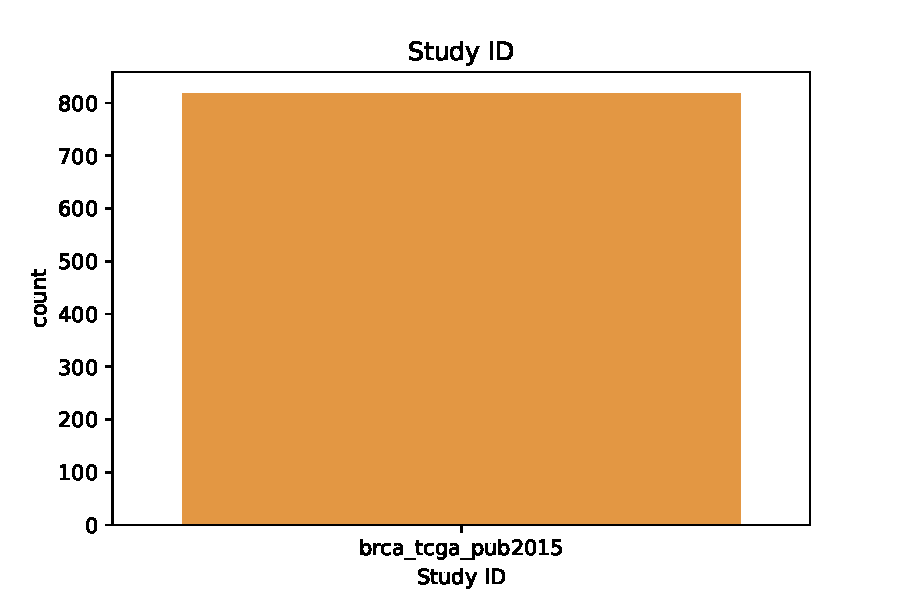
\includegraphics[width=.25\textwidth]{NOTEBOOK/IMAGENES_CRUDAS/1} 
			& 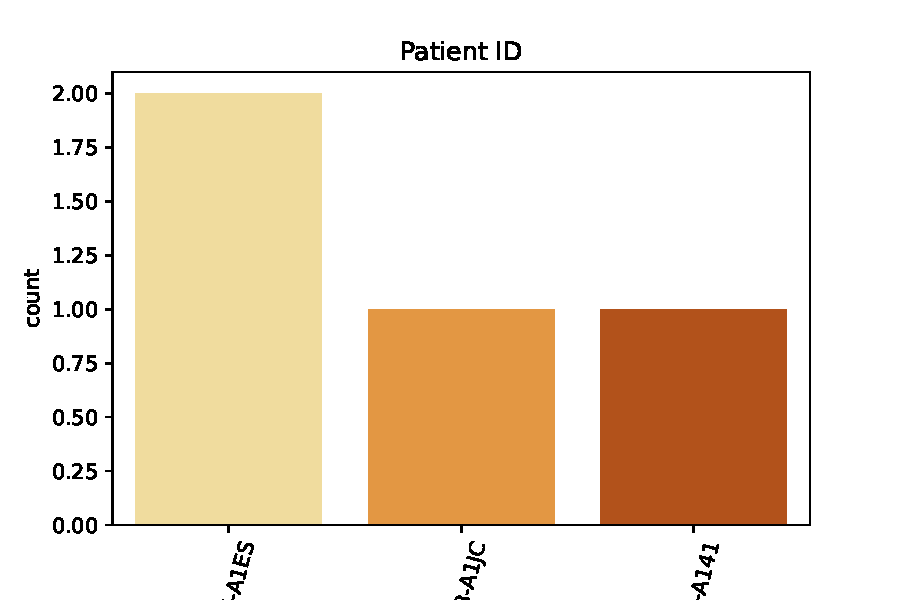
\includegraphics[width=.25\textwidth]{NOTEBOOK/IMAGENES_CRUDAS/2} 
			& 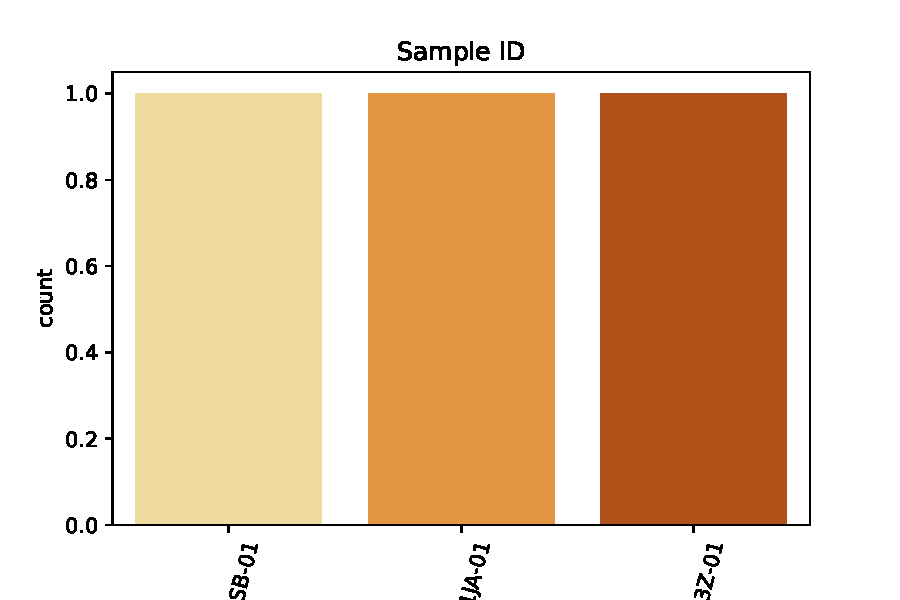
\includegraphics[width=.25\textwidth]{NOTEBOOK/IMAGENES_CRUDAS/3}
			& 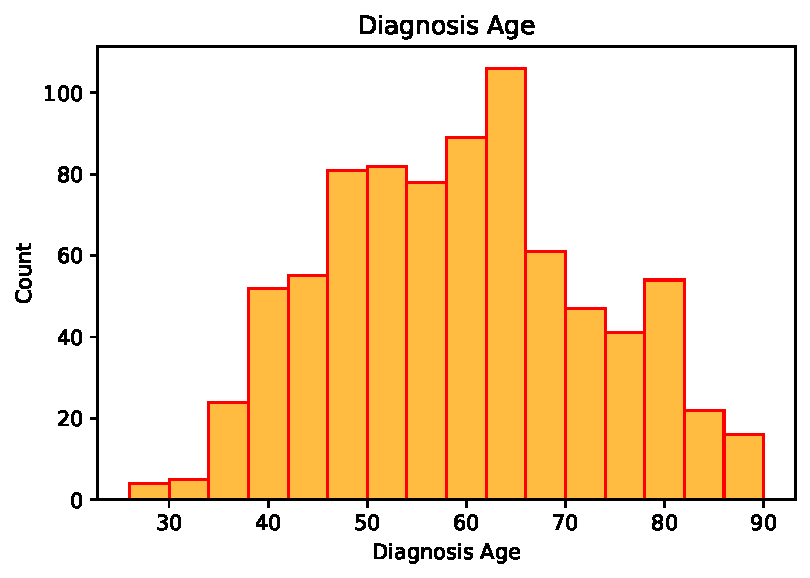
\includegraphics[width=.25\textwidth]{NOTEBOOK/IMAGENES_CRUDAS/4} 
			\\  \hline 
			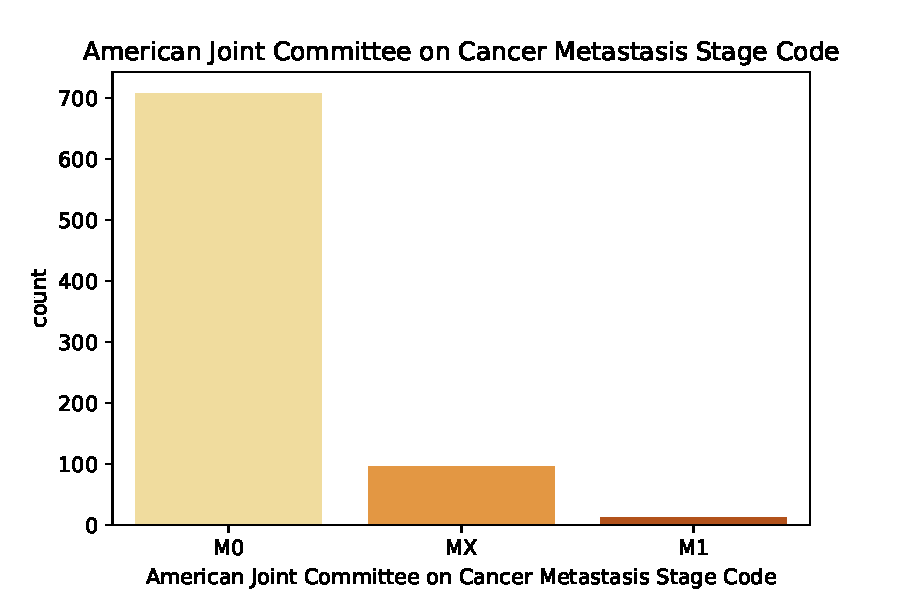
\includegraphics[width=.25\textwidth]{NOTEBOOK/IMAGENES_CRUDAS/5} 
			& 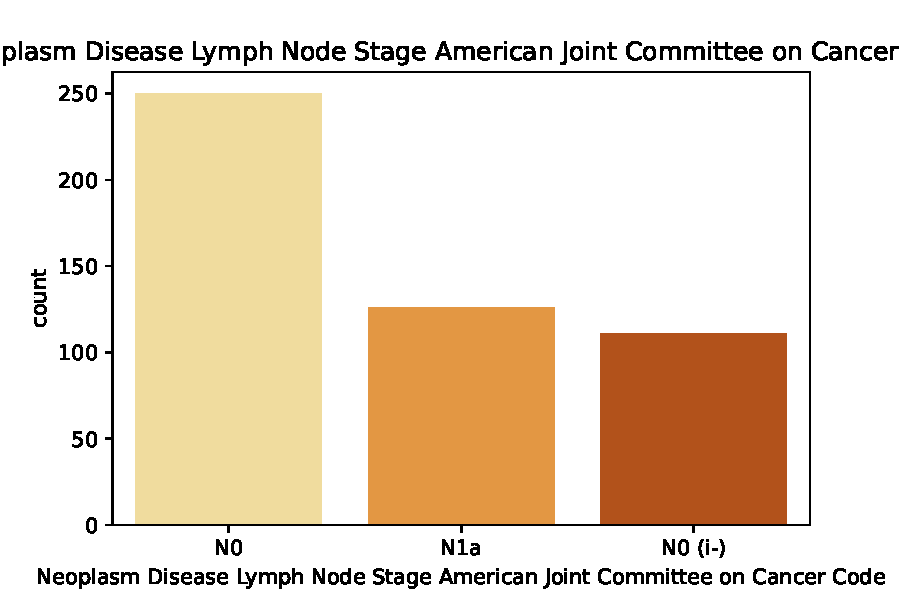
\includegraphics[width=.25\textwidth]{NOTEBOOK/IMAGENES_CRUDAS/6} 
			& 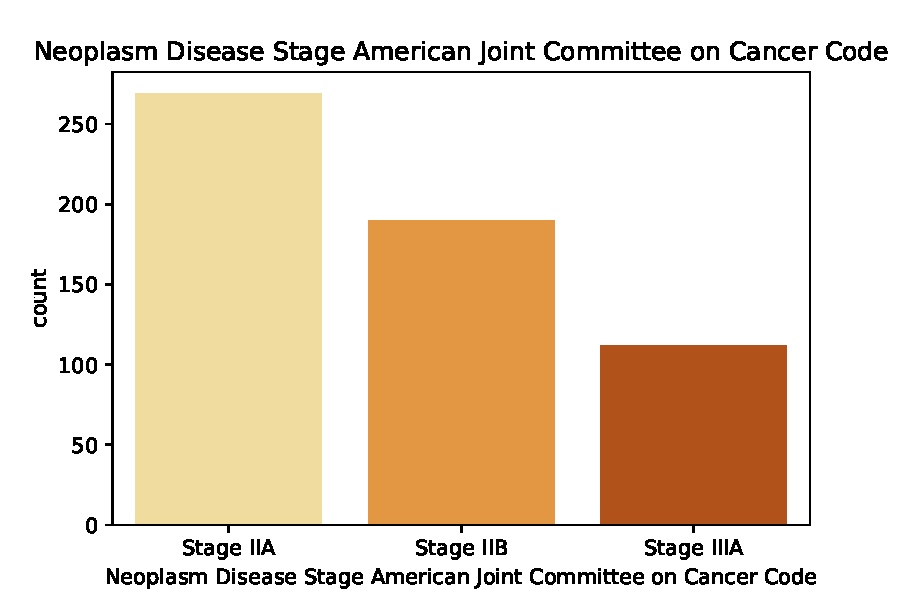
\includegraphics[width=.25\textwidth]{NOTEBOOK/IMAGENES_CRUDAS/7} 
			& 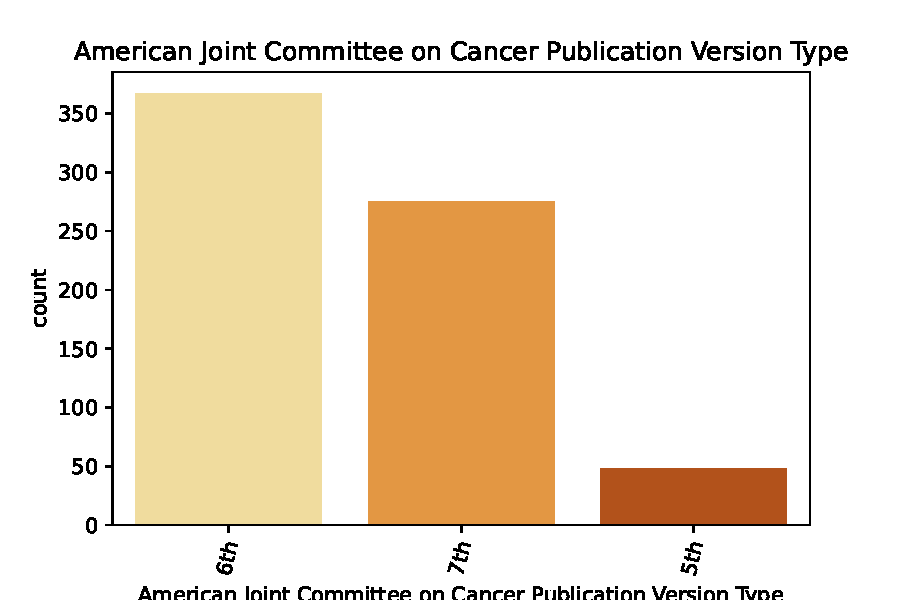
\includegraphics[width=.25\textwidth]{NOTEBOOK/IMAGENES_CRUDAS/8} 
			\\  \hline 
			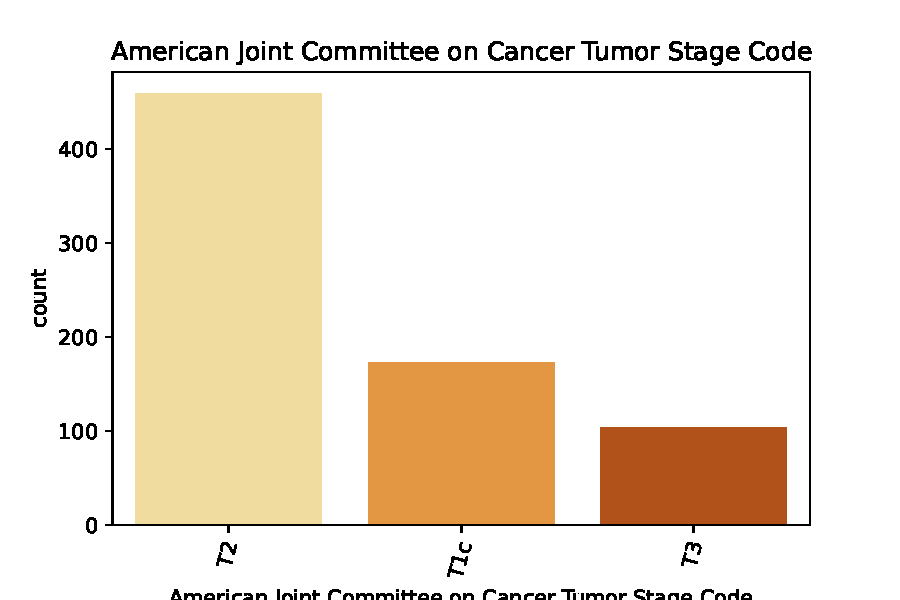
\includegraphics[width=.25\textwidth]{NOTEBOOK/IMAGENES_CRUDAS/9} 
			& 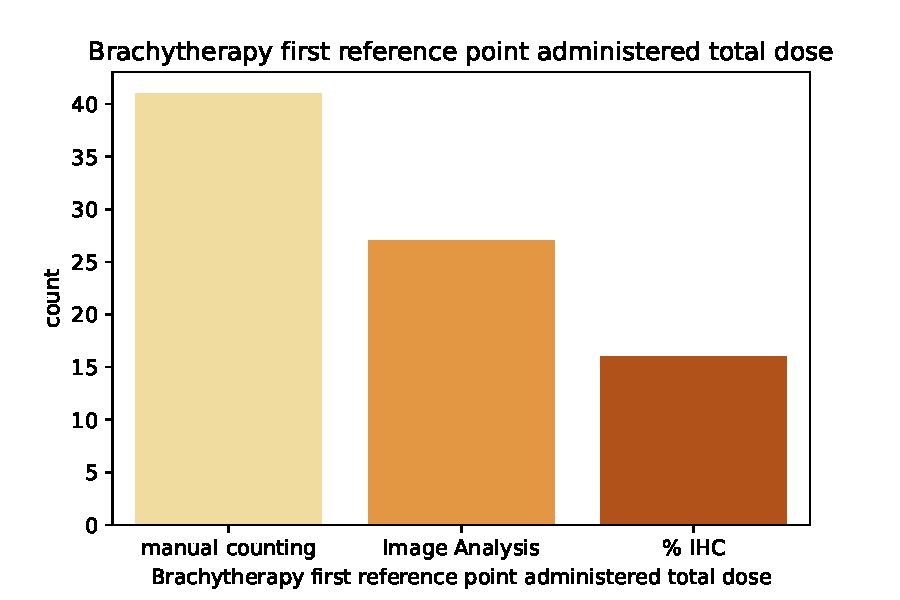
\includegraphics[width=.25\textwidth]{NOTEBOOK/IMAGENES_CRUDAS/10} 
			& 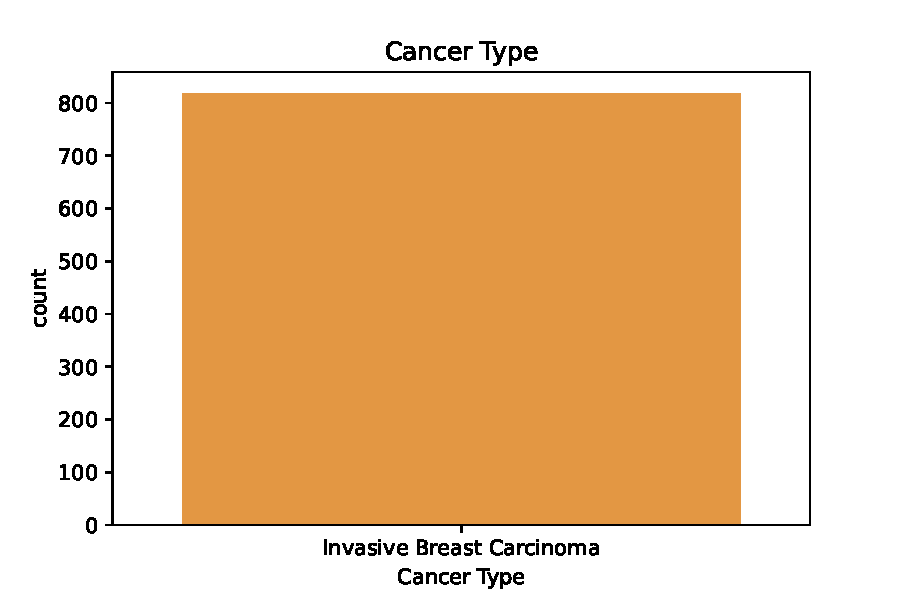
\includegraphics[width=.25\textwidth]{NOTEBOOK/IMAGENES_CRUDAS/11} 
			& 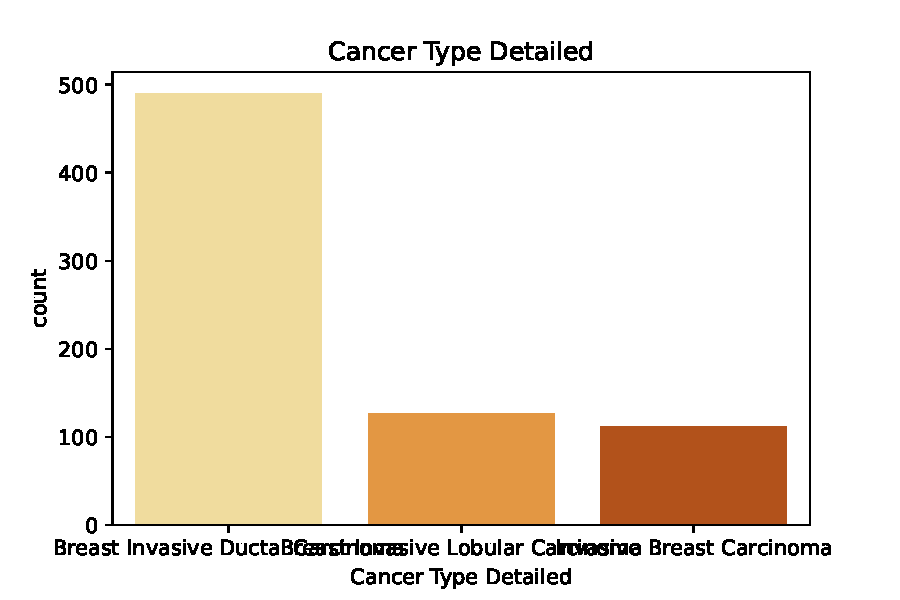
\includegraphics[width=.25\textwidth]{NOTEBOOK/IMAGENES_CRUDAS/12} 
			\\  \hline 
			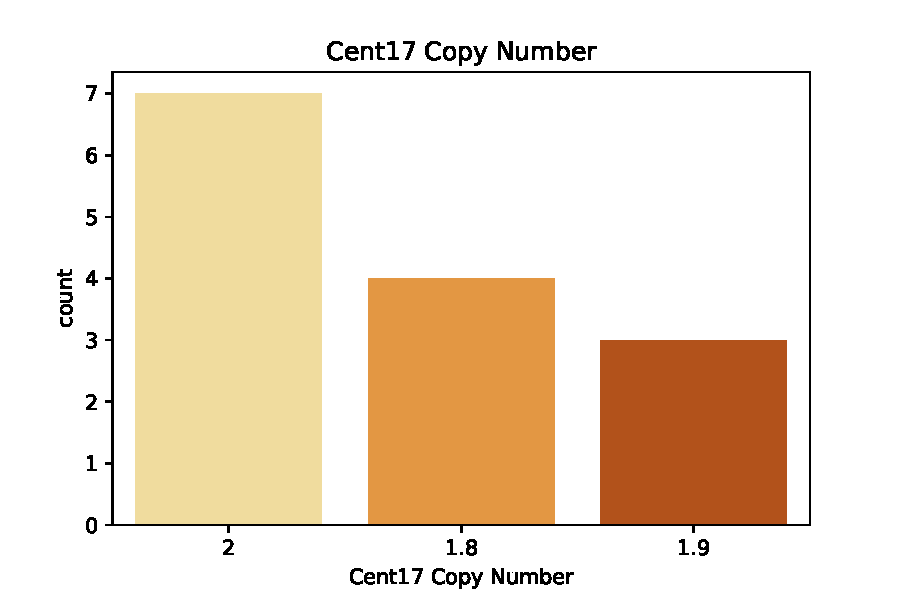
\includegraphics[width=.25\textwidth]{NOTEBOOK/IMAGENES_CRUDAS/13} 
			& 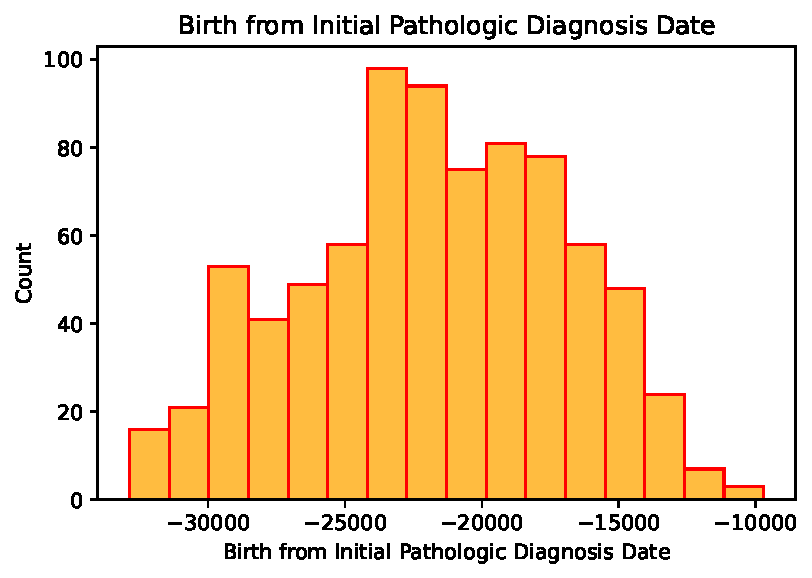
\includegraphics[width=.25\textwidth]{NOTEBOOK/IMAGENES_CRUDAS/14} 
			& 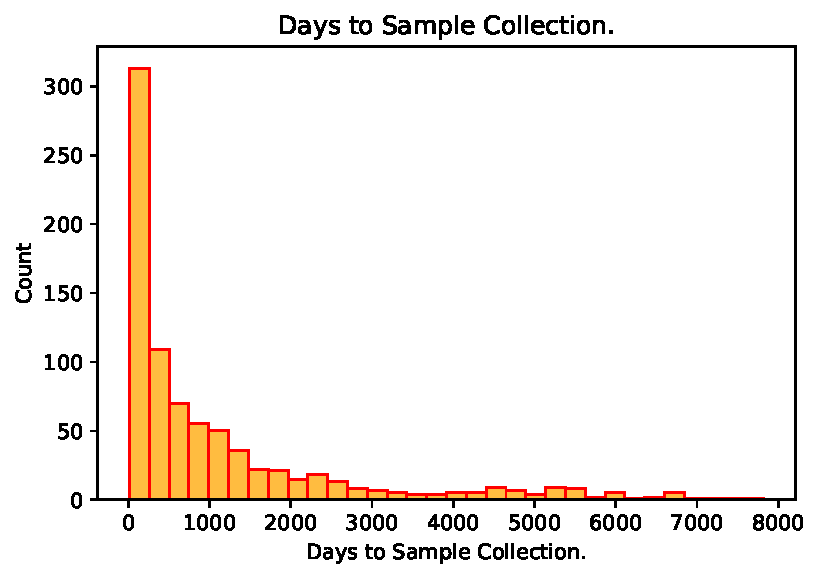
\includegraphics[width=.25\textwidth]{NOTEBOOK/IMAGENES_CRUDAS/15} 
			& 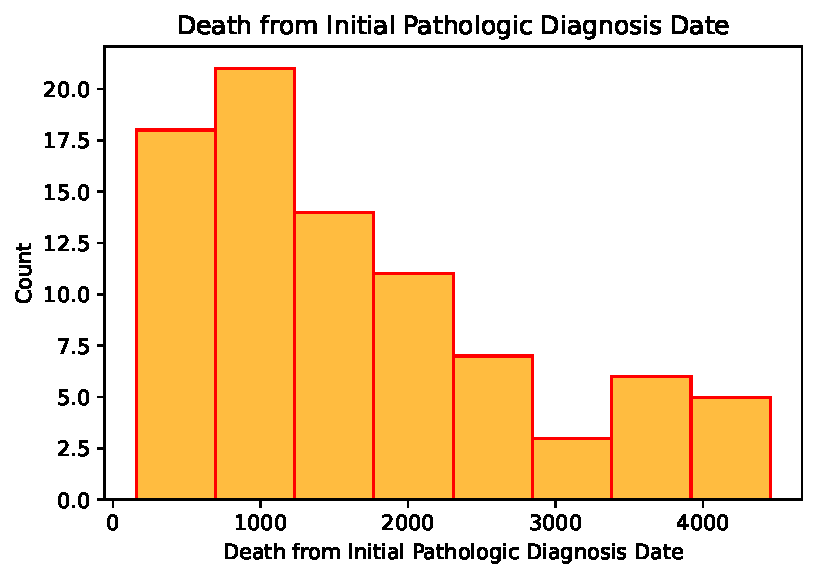
\includegraphics[width=.25\textwidth]{NOTEBOOK/IMAGENES_CRUDAS/16} 
			\\  \hline
			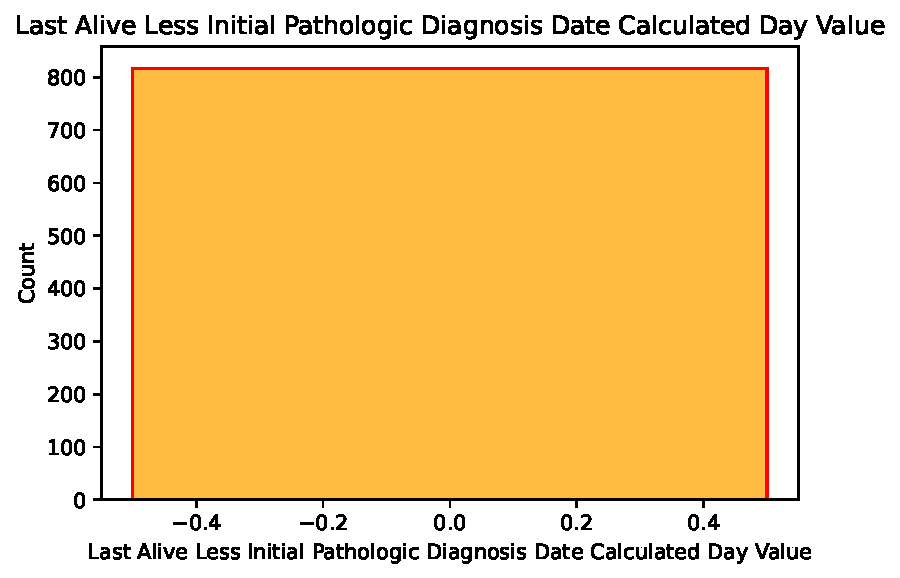
\includegraphics[width=.25\textwidth]{NOTEBOOK/IMAGENES_CRUDAS/17} 
			& 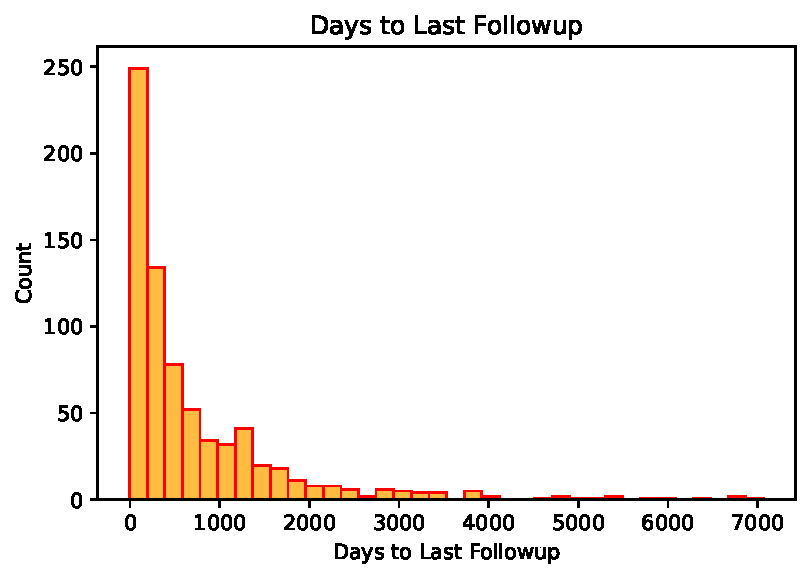
\includegraphics[width=.25\textwidth]{NOTEBOOK/IMAGENES_CRUDAS/18} 
			& 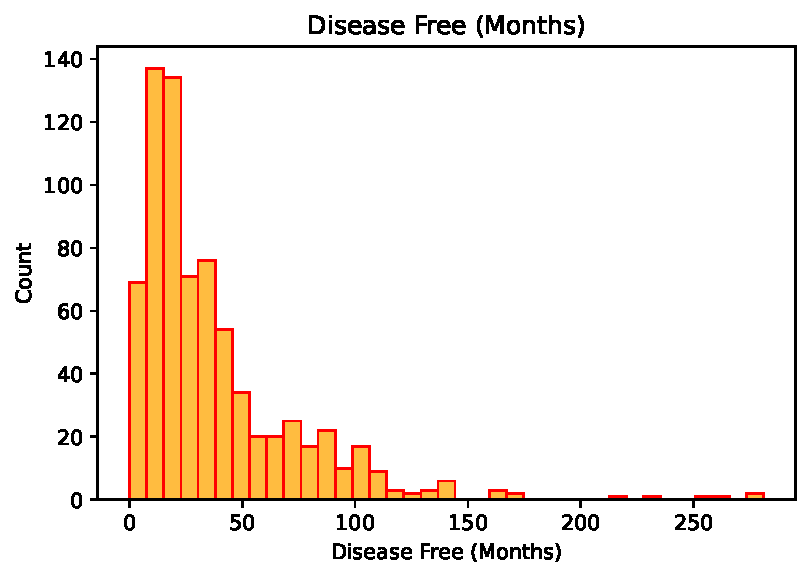
\includegraphics[width=.25\textwidth]{NOTEBOOK/IMAGENES_CRUDAS/19} 
			& 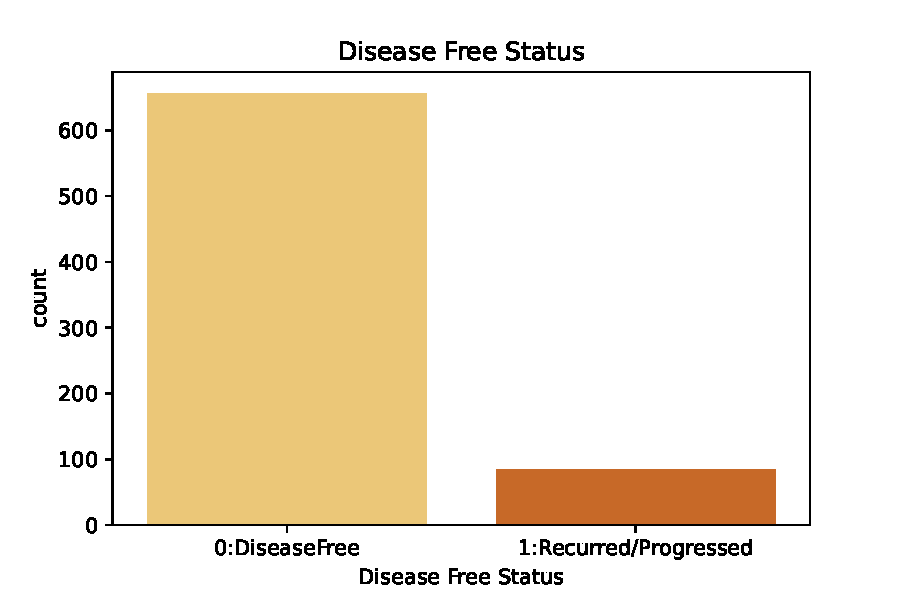
\includegraphics[width=.25\textwidth]{NOTEBOOK/IMAGENES_CRUDAS/20} 
			\\  \hline
			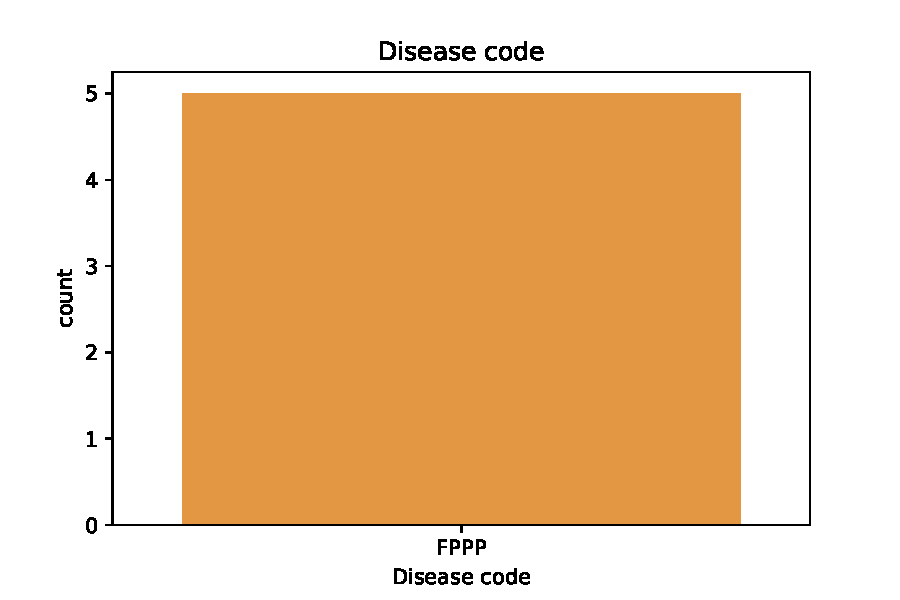
\includegraphics[width=.25\textwidth]{NOTEBOOK/IMAGENES_CRUDAS/21} 
			& 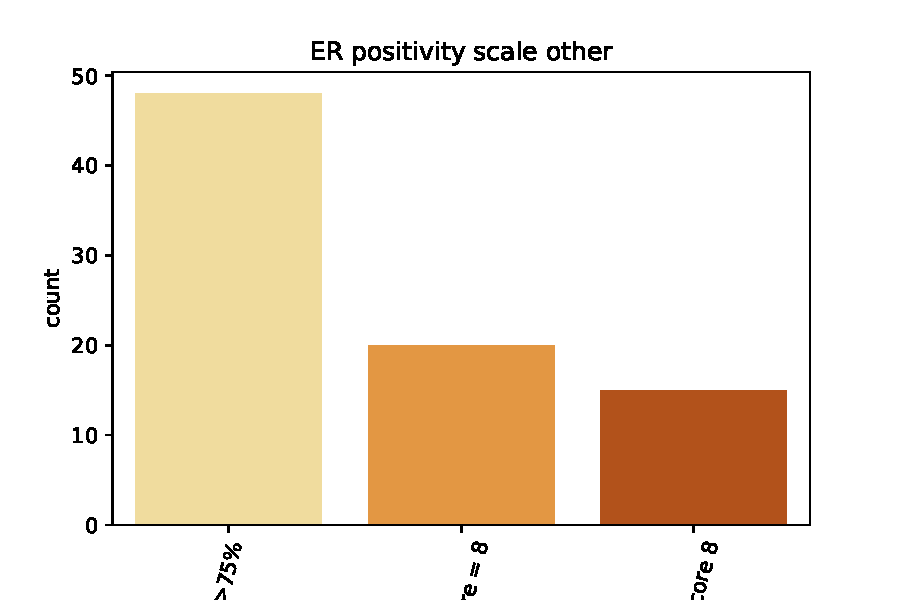
\includegraphics[width=.25\textwidth]{NOTEBOOK/IMAGENES_CRUDAS/22} 
			& 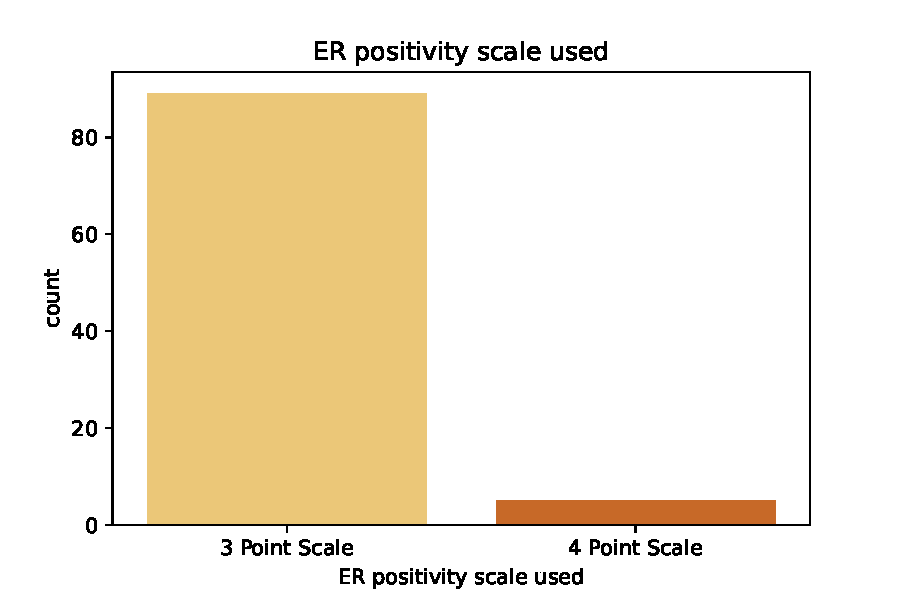
\includegraphics[width=.25\textwidth]{NOTEBOOK/IMAGENES_CRUDAS/23} 
			& 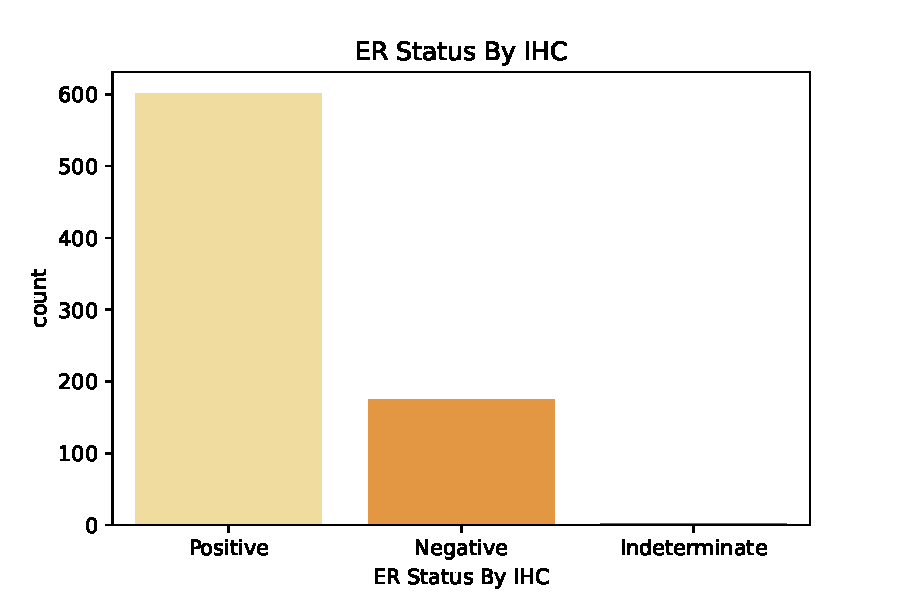
\includegraphics[width=.25\textwidth]{NOTEBOOK/IMAGENES_CRUDAS/24} 
			\\  \hline 
			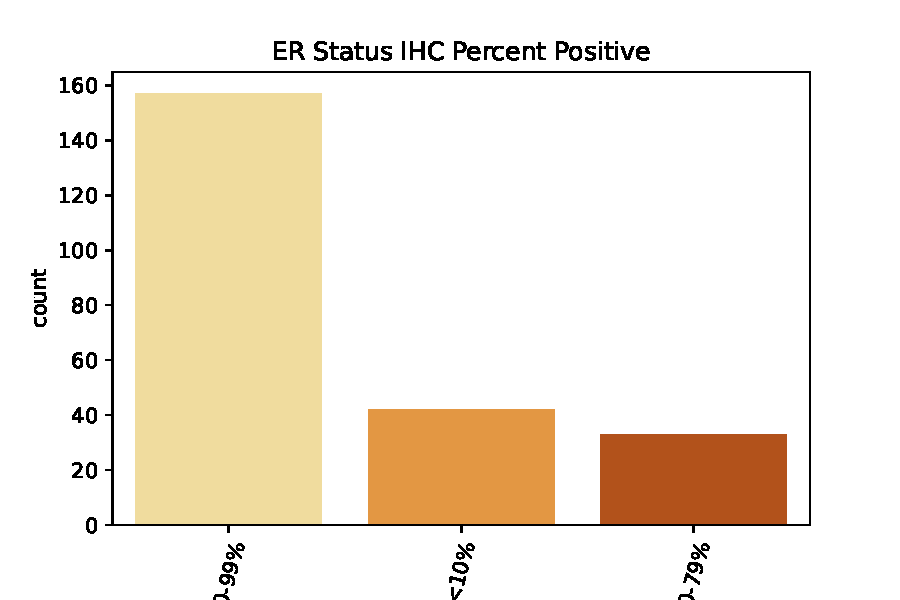
\includegraphics[width=.25\textwidth]{NOTEBOOK/IMAGENES_CRUDAS/25} 
			& 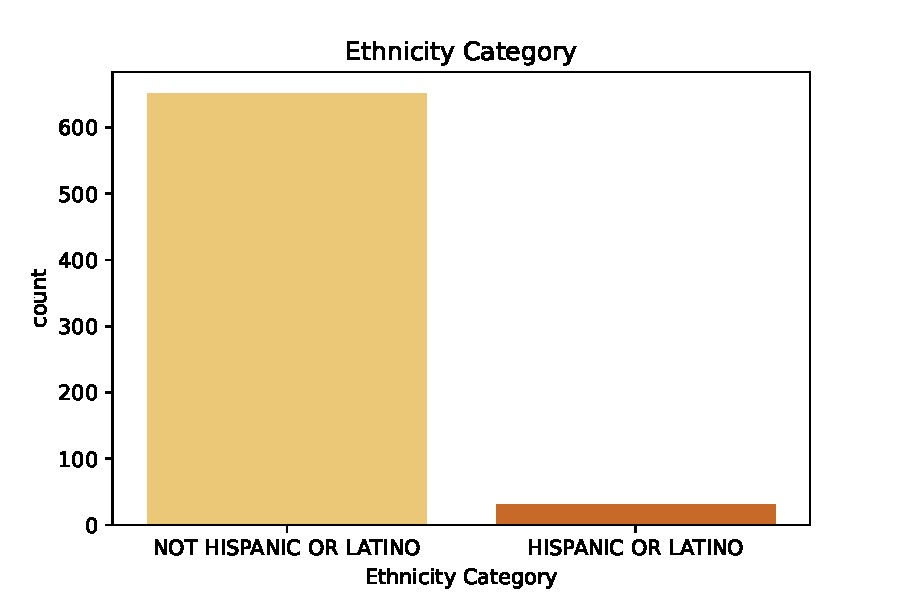
\includegraphics[width=.25\textwidth]{NOTEBOOK/IMAGENES_CRUDAS/26} 
			& 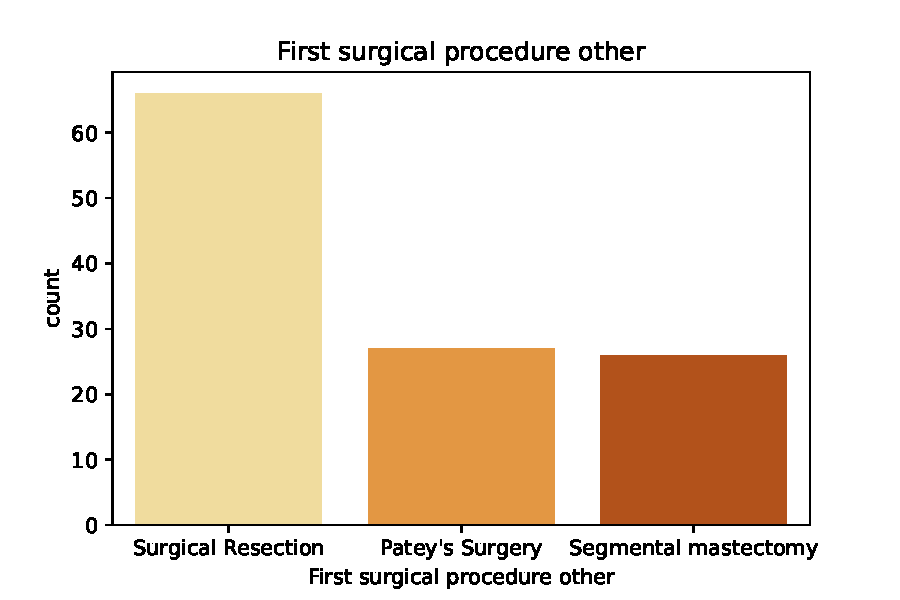
\includegraphics[width=.25\textwidth]{NOTEBOOK/IMAGENES_CRUDAS/27} 
			& 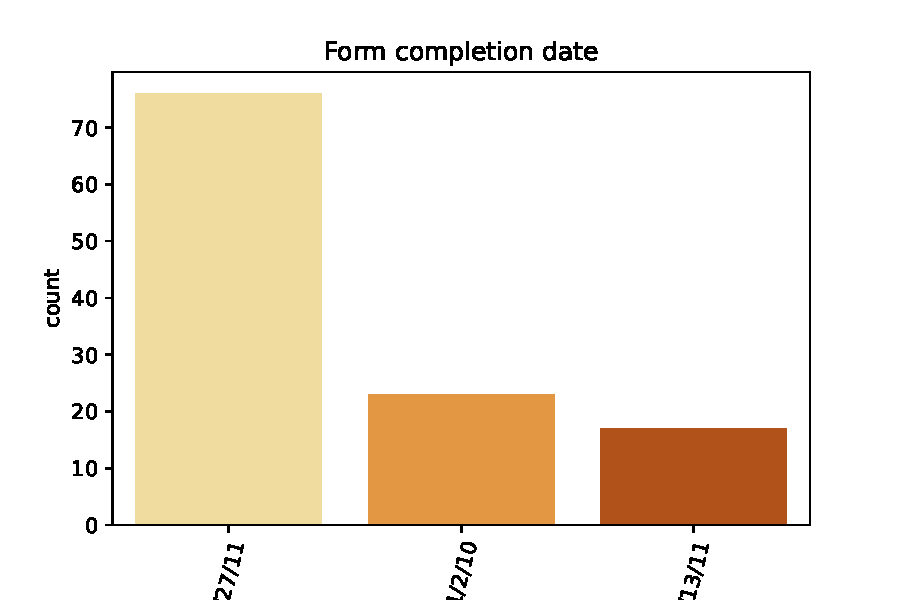
\includegraphics[width=.25\textwidth]{NOTEBOOK/IMAGENES_CRUDAS/28}   
			\\  \hline                
		\end{tabular} 
	\end{center} 
\end{table}

\clearpage
\begin{center} 
	\begin{tabular}{ |c|c|c|c| }  
		\hline 
		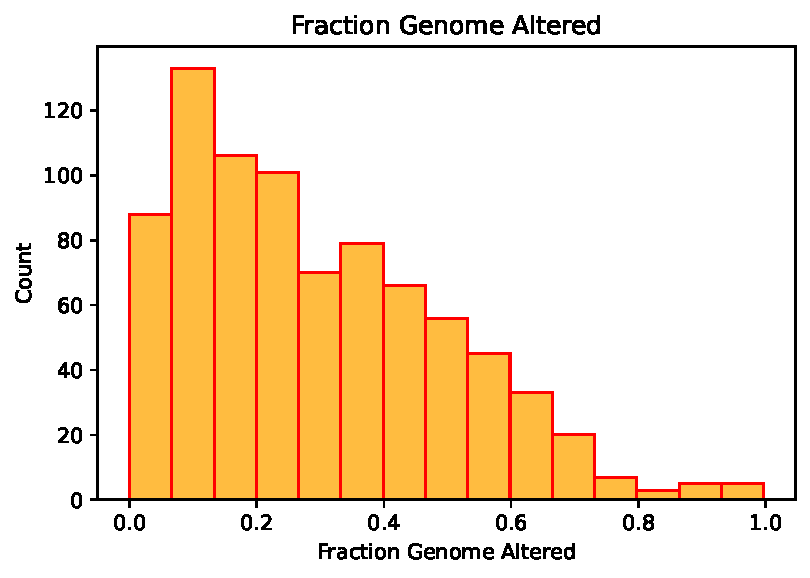
\includegraphics[width=.25\textwidth]{NOTEBOOK/IMAGENES_CRUDAS/29} 
		& 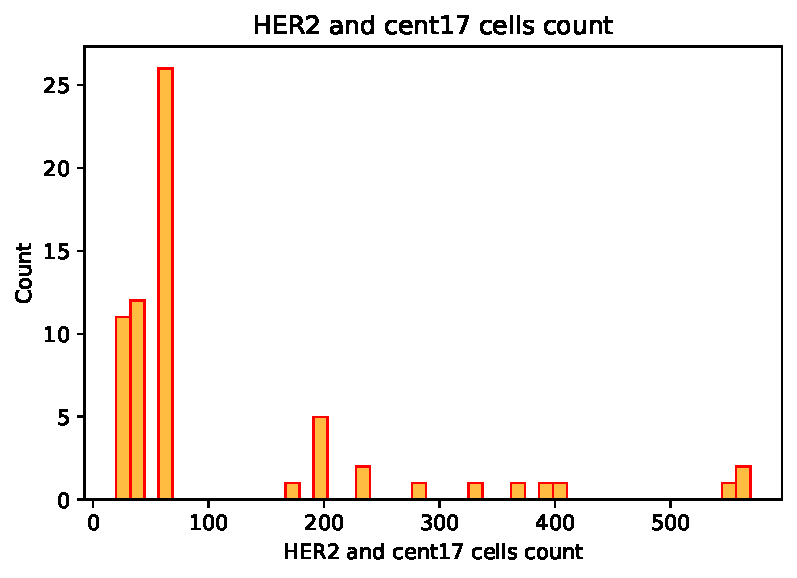
\includegraphics[width=.25\textwidth]{NOTEBOOK/IMAGENES_CRUDAS/30} 
		& 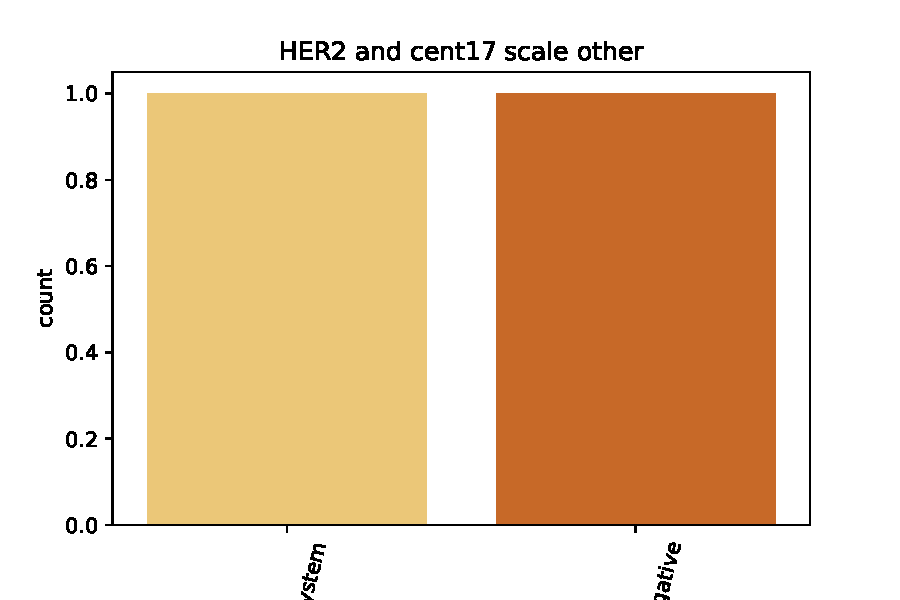
\includegraphics[width=.25\textwidth]{NOTEBOOK/IMAGENES_CRUDAS/31} 
		& 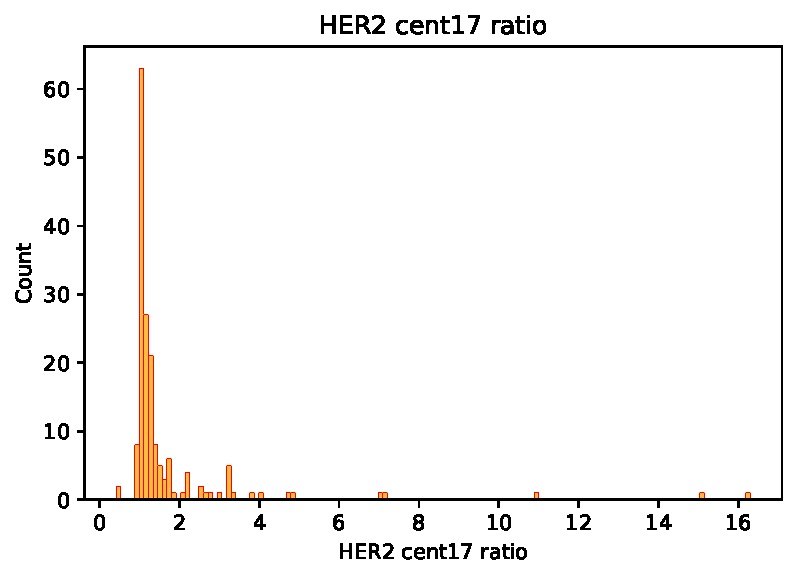
\includegraphics[width=.25\textwidth]{NOTEBOOK/IMAGENES_CRUDAS/32}   
		\\  \hline   
		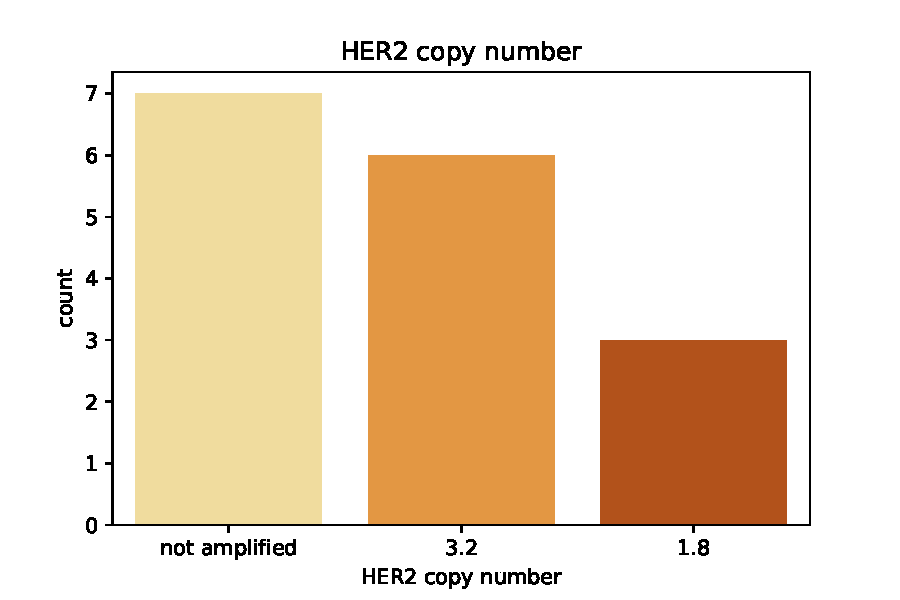
\includegraphics[width=.22\textwidth]{NOTEBOOK/IMAGENES_CRUDAS/33} 
		& 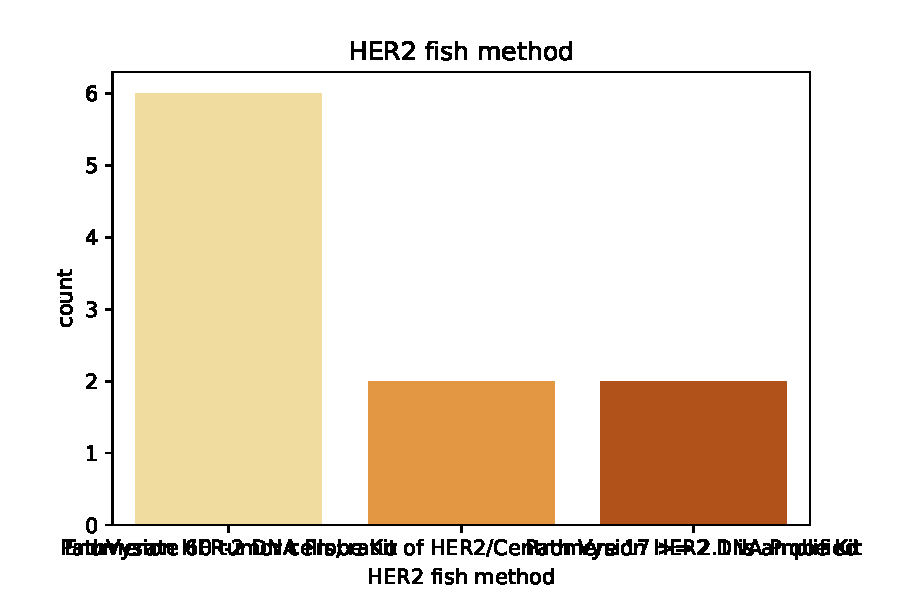
\includegraphics[width=.25\textwidth]{NOTEBOOK/IMAGENES_CRUDAS/34}
		& 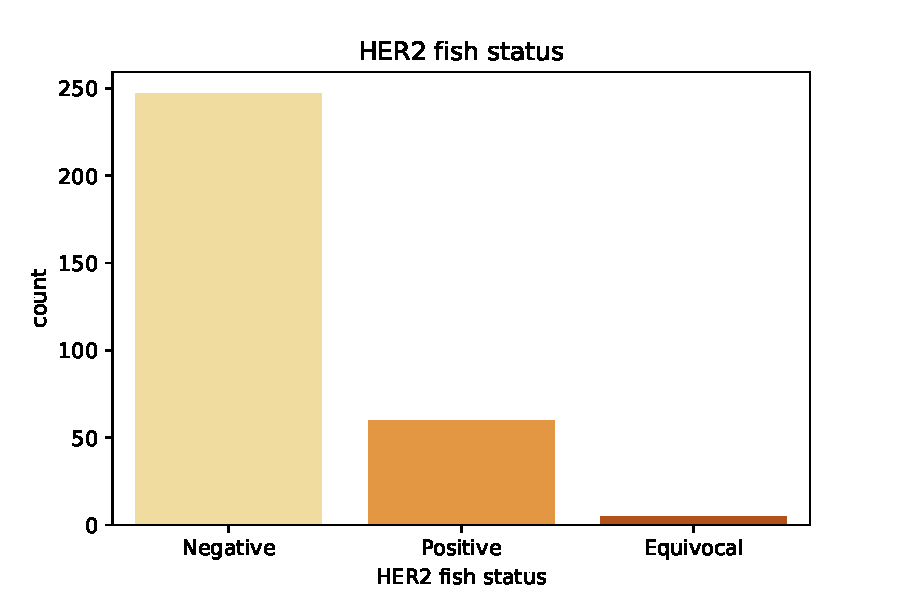
\includegraphics[width=.25\textwidth]{NOTEBOOK/IMAGENES_CRUDAS/35}
		& 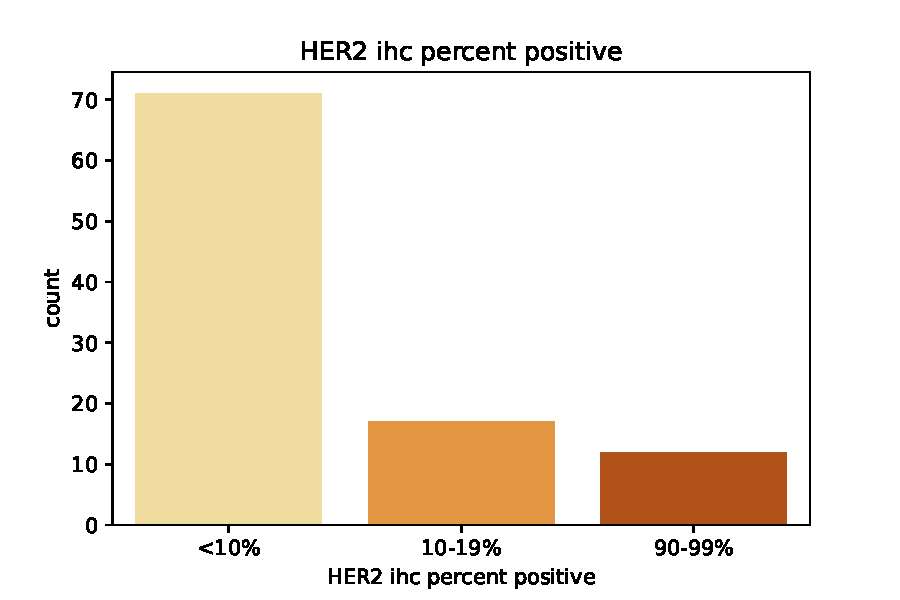
\includegraphics[width=.25\textwidth]{NOTEBOOK/IMAGENES_CRUDAS/36} 
		\\  \hline 
		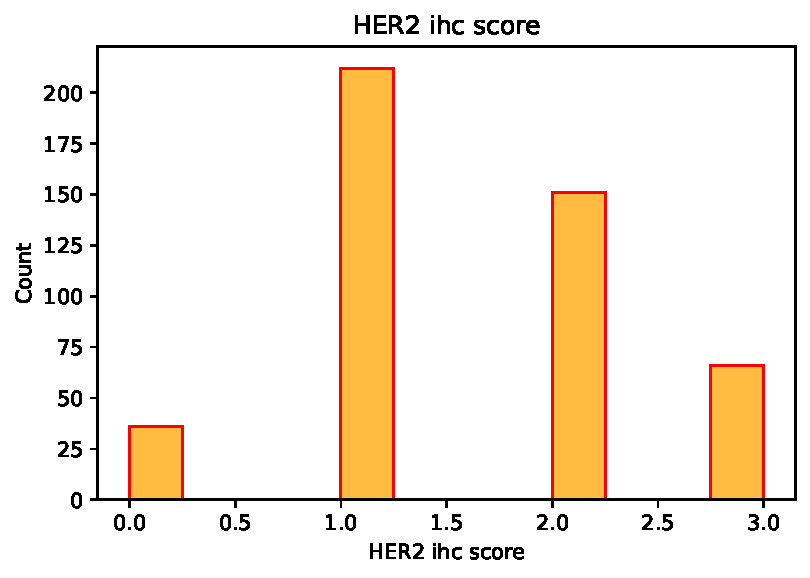
\includegraphics[width=.25\textwidth]{NOTEBOOK/IMAGENES_CRUDAS/37} 
		& 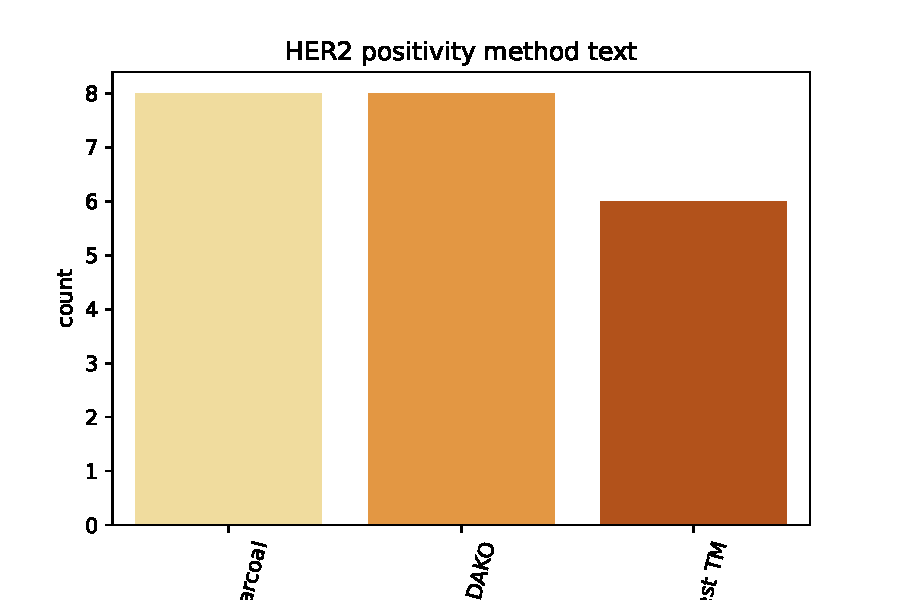
\includegraphics[width=.25\textwidth]{NOTEBOOK/IMAGENES_CRUDAS/38} 
		& 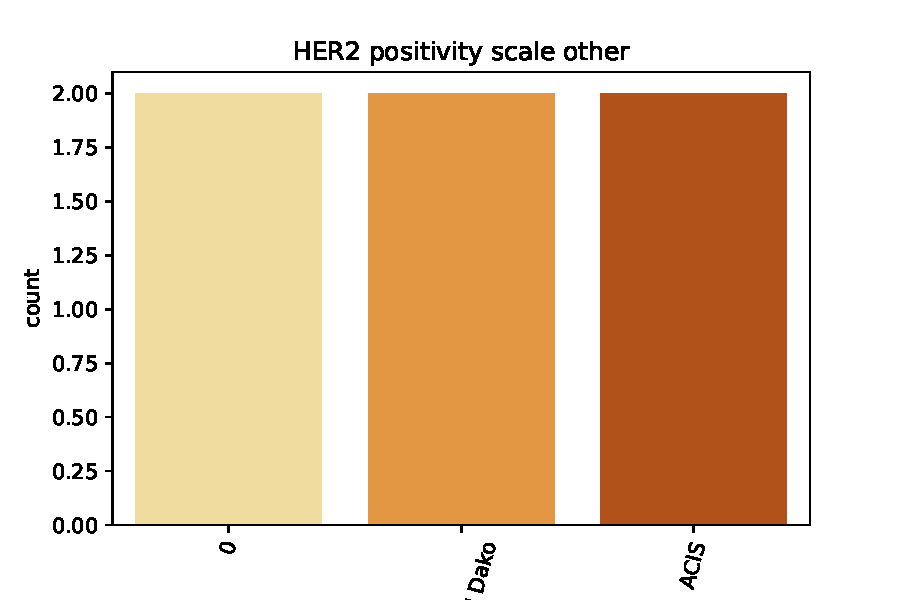
\includegraphics[width=.25\textwidth]{NOTEBOOK/IMAGENES_CRUDAS/39} 
		& 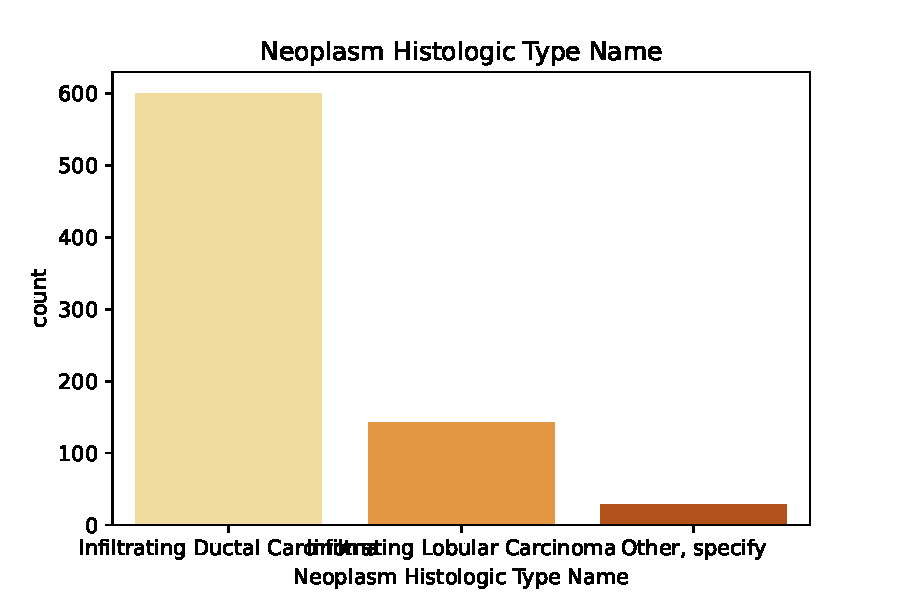
\includegraphics[width=.25\textwidth]{NOTEBOOK/IMAGENES_CRUDAS/40} 
		\\  \hline 
		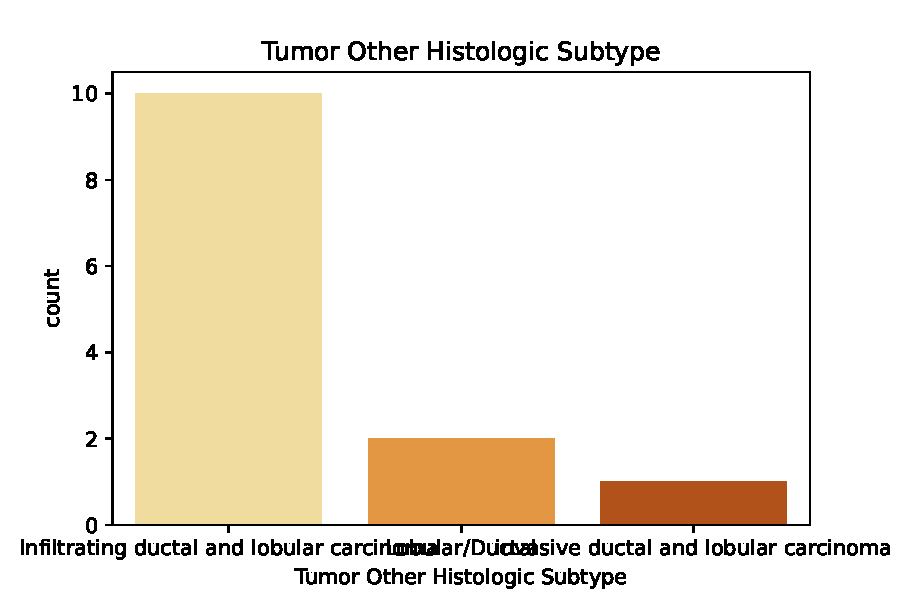
\includegraphics[width=.25\textwidth]{NOTEBOOK/IMAGENES_CRUDAS/41} 
		& 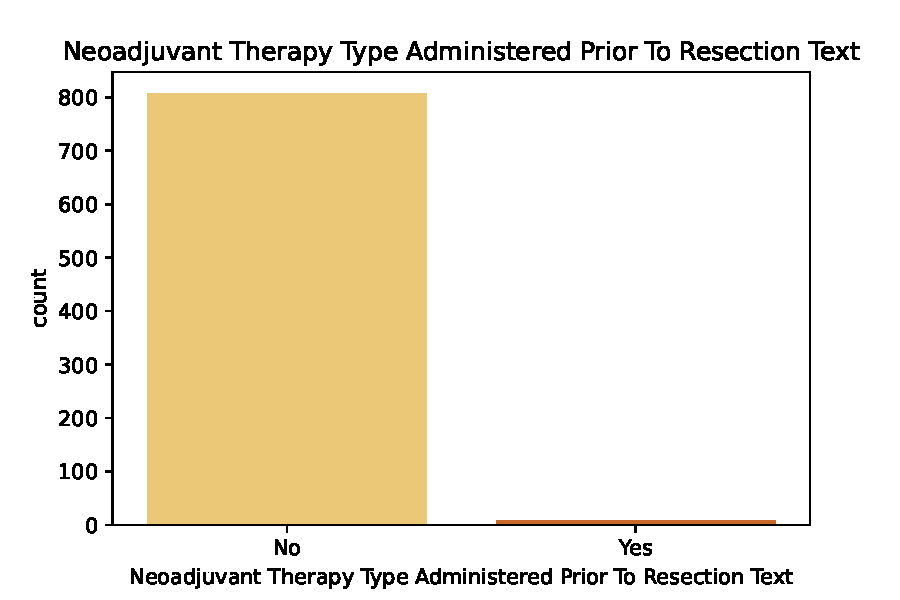
\includegraphics[width=.25\textwidth]{NOTEBOOK/IMAGENES_CRUDAS/42} 
		& 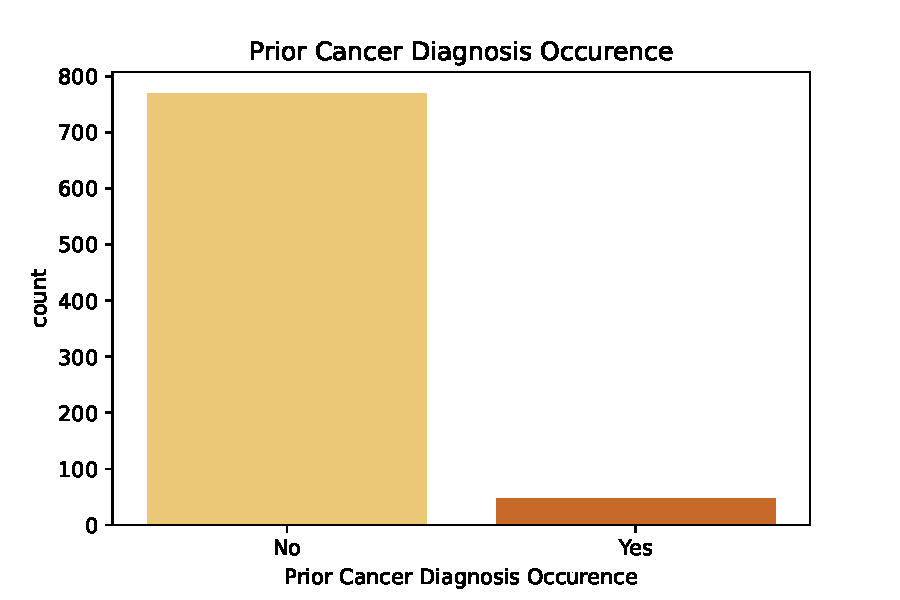
\includegraphics[width=.25\textwidth]{NOTEBOOK/IMAGENES_CRUDAS/43} 
		& 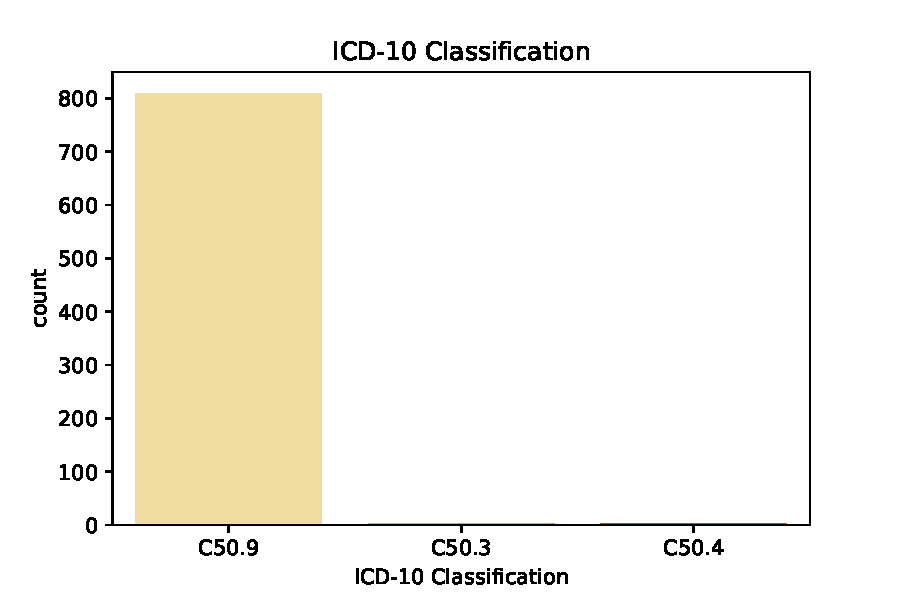
\includegraphics[width=.25\textwidth]{NOTEBOOK/IMAGENES_CRUDAS/44} 
		\\  \hline 
		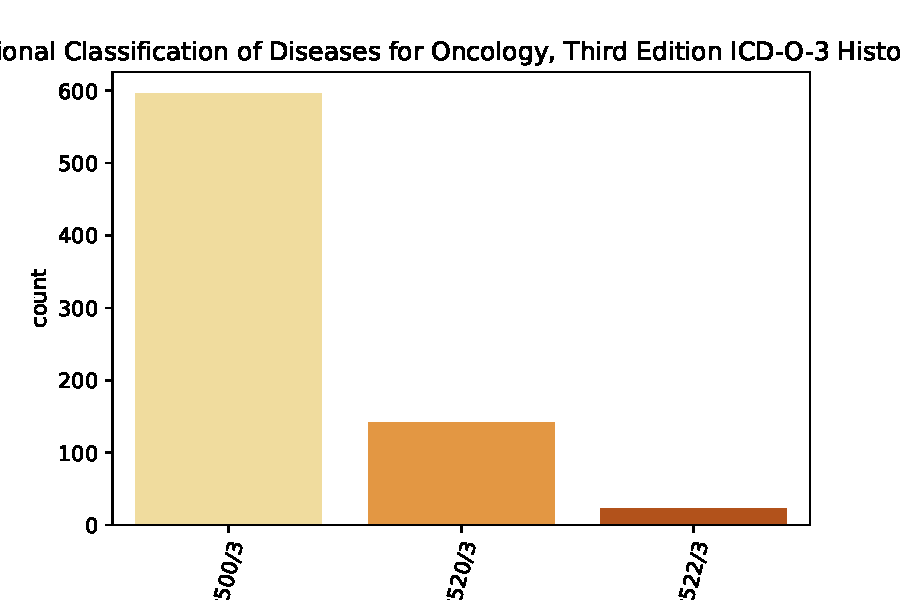
\includegraphics[width=.25\textwidth]{NOTEBOOK/IMAGENES_CRUDAS/45} 
		& 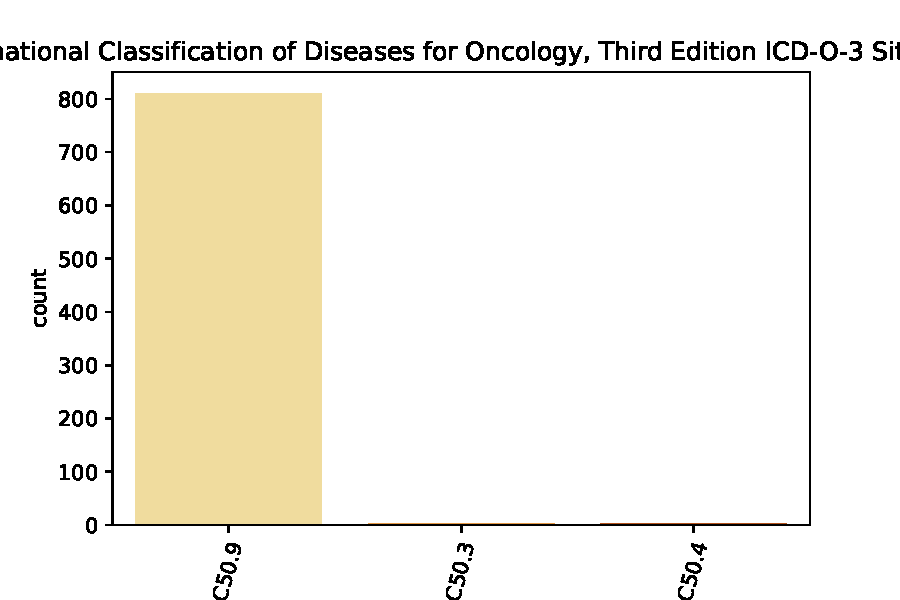
\includegraphics[width=.25\textwidth]{NOTEBOOK/IMAGENES_CRUDAS/46} 
		& 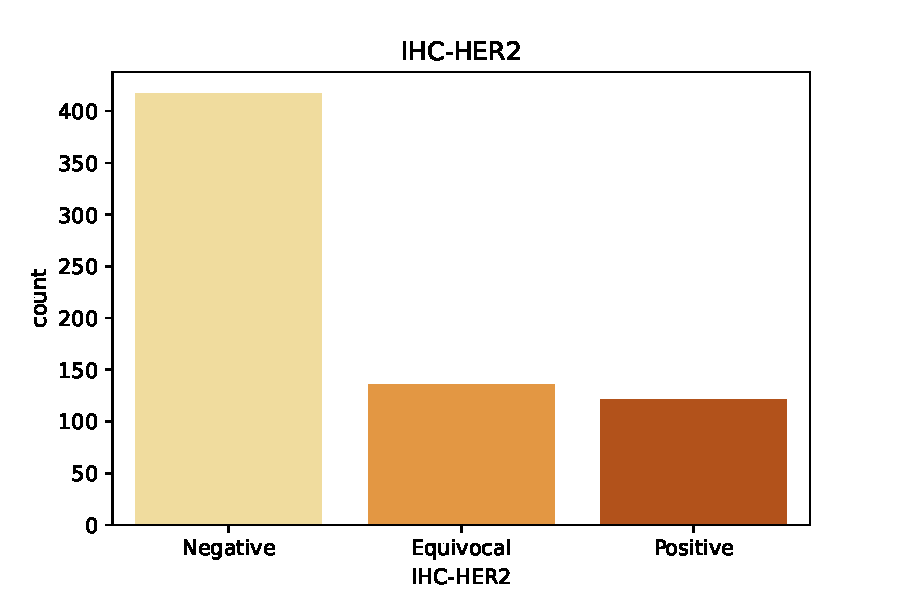
\includegraphics[width=.25\textwidth]{NOTEBOOK/IMAGENES_CRUDAS/47} 
		& 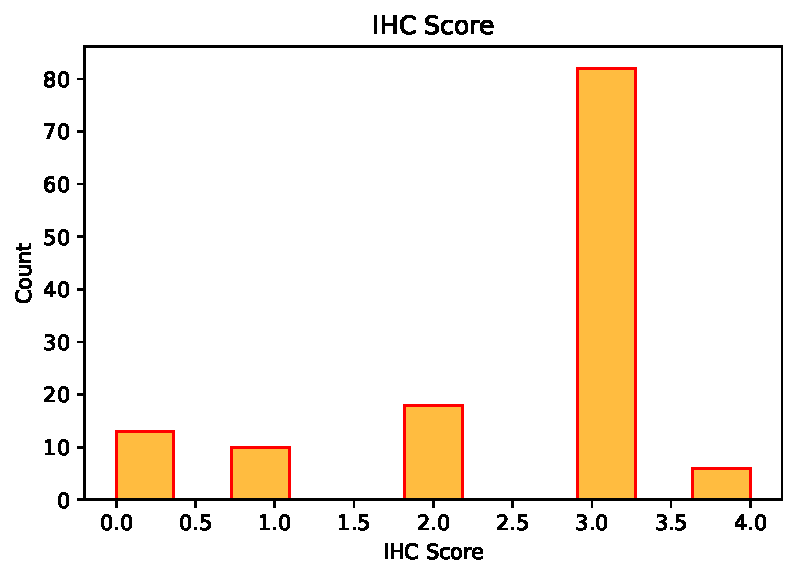
\includegraphics[width=.25\textwidth]{NOTEBOOK/IMAGENES_CRUDAS/48} 
		\\  \hline
		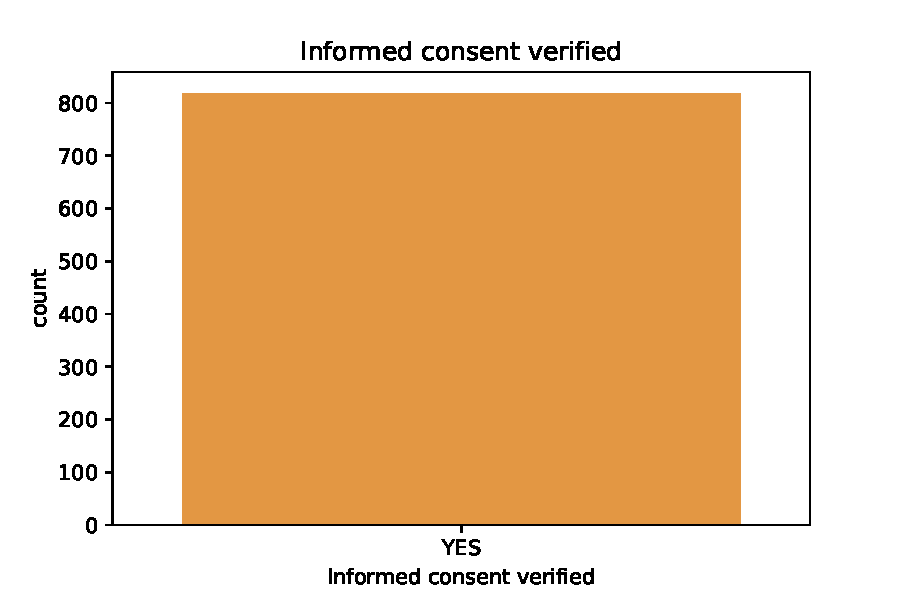
\includegraphics[width=.25\textwidth]{NOTEBOOK/IMAGENES_CRUDAS/49} 
		& 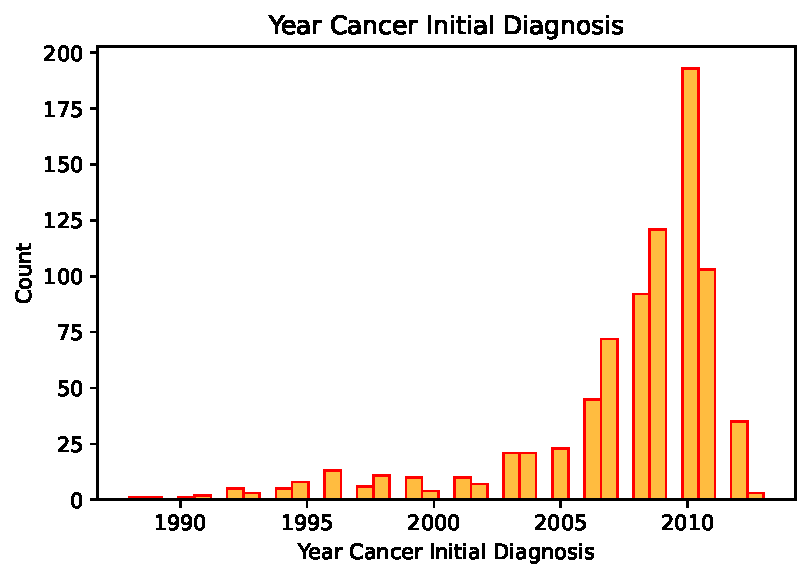
\includegraphics[width=.25\textwidth]{NOTEBOOK/IMAGENES_CRUDAS/50} 
		& \includegraphics[width=.25\textwidth]{NOTEBOOK/IMAGENES_CRUDAS/51} 
		& \includegraphics[width=.25\textwidth]{NOTEBOOK/IMAGENES_CRUDAS/52} 
		\\  \hline
		\includegraphics[width=.25\textwidth]{NOTEBOOK/IMAGENES_CRUDAS/53} 
		& \includegraphics[width=.25\textwidth]{NOTEBOOK/IMAGENES_CRUDAS/54} 
		& \includegraphics[width=.25\textwidth]{NOTEBOOK/IMAGENES_CRUDAS/55} 
		& \includegraphics[width=.25\textwidth]{NOTEBOOK/IMAGENES_CRUDAS/56} 
		\\  \hline         
	\end{tabular} 
\end{center} 

\begin{center} 
	\begin{tabular}{ |c|c|c|c| } 
		\hline 
		\includegraphics[width=.25\textwidth]{NOTEBOOK/IMAGENES_CRUDAS/57} 
		& \includegraphics[width=.25\textwidth]{NOTEBOOK/IMAGENES_CRUDAS/58} 
		& \includegraphics[width=.25\textwidth]{NOTEBOOK/IMAGENES_CRUDAS/59} 
		& \includegraphics[width=.25\textwidth]{NOTEBOOK/IMAGENES_CRUDAS/60}   
		\\  \hline       
		\hline 
		\includegraphics[width=.25\textwidth]{NOTEBOOK/IMAGENES_CRUDAS/61} 
		& \includegraphics[width=.25\textwidth]{NOTEBOOK/IMAGENES_CRUDAS/62} 
		& \includegraphics[width=.25\textwidth]{NOTEBOOK/IMAGENES_CRUDAS/63} 
		& \includegraphics[width=.25\textwidth]{NOTEBOOK/IMAGENES_CRUDAS/64}   
		\\  \hline    
		\includegraphics[width=.22\textwidth]{NOTEBOOK/IMAGENES_CRUDAS/65} 
		& \includegraphics[width=.25\textwidth]{NOTEBOOK/IMAGENES_CRUDAS/66}
		& \includegraphics[width=.25\textwidth]{NOTEBOOK/IMAGENES_CRUDAS/67}
		& \includegraphics[width=.25\textwidth]{NOTEBOOK/IMAGENES_CRUDAS/68} 
		\\  \hline 
		\includegraphics[width=.25\textwidth]{NOTEBOOK/IMAGENES_CRUDAS/69} 
		& \includegraphics[width=.25\textwidth]{NOTEBOOK/IMAGENES_CRUDAS/70} 
		& \includegraphics[width=.25\textwidth]{NOTEBOOK/IMAGENES_CRUDAS/71} 
		& \includegraphics[width=.25\textwidth]{NOTEBOOK/IMAGENES_CRUDAS/72} 
		\\  \hline 
		\includegraphics[width=.25\textwidth]{NOTEBOOK/IMAGENES_CRUDAS/73} 
		& \includegraphics[width=.25\textwidth]{NOTEBOOK/IMAGENES_CRUDAS/74} 
		& \includegraphics[width=.25\textwidth]{NOTEBOOK/IMAGENES_CRUDAS/75} 
		& \includegraphics[width=.25\textwidth]{NOTEBOOK/IMAGENES_CRUDAS/76} 
		\\  \hline 
		\includegraphics[width=.25\textwidth]{NOTEBOOK/IMAGENES_CRUDAS/77} 
		& \includegraphics[width=.25\textwidth]{NOTEBOOK/IMAGENES_CRUDAS/78} 
		& \includegraphics[width=.25\textwidth]{NOTEBOOK/IMAGENES_CRUDAS/79} 
		& \includegraphics[width=.25\textwidth]{NOTEBOOK/IMAGENES_CRUDAS/80} 
		\\  \hline
		\includegraphics[width=.25\textwidth]{NOTEBOOK/IMAGENES_CRUDAS/81} 
		& \includegraphics[width=.25\textwidth]{NOTEBOOK/IMAGENES_CRUDAS/82} 
		& \includegraphics[width=.25\textwidth]{NOTEBOOK/IMAGENES_CRUDAS/83} 
		& \includegraphics[width=.25\textwidth]{NOTEBOOK/IMAGENES_CRUDAS/84} 
		\\  \hline           
	\end{tabular} 
\end{center} 

\begin{center} 
	\begin{tabular}{ |c|c|c|c| }  
		\hline
		\includegraphics[width=.25\textwidth]{NOTEBOOK/IMAGENES_CRUDAS/85} 
		& \includegraphics[width=.25\textwidth]{NOTEBOOK/IMAGENES_CRUDAS/86} 
		& \includegraphics[width=.25\textwidth]{NOTEBOOK/IMAGENES_CRUDAS/87} 
		& \includegraphics[width=.25\textwidth]{NOTEBOOK/IMAGENES_CRUDAS/88} 
		\\  \hline 
		\includegraphics[width=.25\textwidth]{NOTEBOOK/IMAGENES_CRUDAS/89} 
		& \includegraphics[width=.25\textwidth]{NOTEBOOK/IMAGENES_CRUDAS/90} 
		& \includegraphics[width=.25\textwidth]{NOTEBOOK/IMAGENES_CRUDAS/91} 
		& \includegraphics[width=.25\textwidth]{NOTEBOOK/IMAGENES_CRUDAS/92}   
		\\  \hline    
		\includegraphics[width=.25\textwidth]{NOTEBOOK/IMAGENES_CRUDAS/93} 
		& \includegraphics[width=.25\textwidth]{NOTEBOOK/IMAGENES_CRUDAS/94} 
		& \includegraphics[width=.25\textwidth]{NOTEBOOK/IMAGENES_CRUDAS/95} 
		& \includegraphics[width=.25\textwidth]{NOTEBOOK/IMAGENES_CRUDAS/96}   
		\\  \hline     
		\includegraphics[width=.22\textwidth]{NOTEBOOK/IMAGENES_CRUDAS/97} 
		& \includegraphics[width=.25\textwidth]{NOTEBOOK/IMAGENES_CRUDAS/98}
		& \includegraphics[width=.25\textwidth]{NOTEBOOK/IMAGENES_CRUDAS/99}
		& \includegraphics[width=.25\textwidth]{NOTEBOOK/IMAGENES_CRUDAS/100} 
		\\  \hline 
		\includegraphics[width=.25\textwidth]{NOTEBOOK/IMAGENES_CRUDAS/101} 
		& \includegraphics[width=.25\textwidth]{NOTEBOOK/IMAGENES_CRUDAS/102} 
		& \includegraphics[width=.25\textwidth]{NOTEBOOK/IMAGENES_CRUDAS/103} 
		& \includegraphics[width=.25\textwidth]{NOTEBOOK/IMAGENES_CRUDAS/104} 
		\\  \hline 
		\includegraphics[width=.25\textwidth]{NOTEBOOK/IMAGENES_CRUDAS/105} 
		& \includegraphics[width=.25\textwidth]{NOTEBOOK/IMAGENES_CRUDAS/106} 
		& \includegraphics[width=.25\textwidth]{NOTEBOOK/IMAGENES_CRUDAS/107} 
		& \includegraphics[width=.25\textwidth]{NOTEBOOK/IMAGENES_CRUDAS/108} 
		\\  \hline                
	\end{tabular} 
	\begin{tabular}{ |c|c| }  
		\hline 
		\includegraphics[width=.22\textwidth]{NOTEBOOK/IMAGENES_CRUDAS/109} 
		& \includegraphics[width=.25\textwidth]{NOTEBOOK/IMAGENES_CRUDAS/110}
		\\  \hline 
	\end{tabular} 
\end{center} 

\newpage
\begin{figure}[!htb]
	\centering
	\includegraphics[width=1
	\linewidth]{NOTEBOOK/IMAGENES_PERDIDAS/missing_displot}
	\caption{Datos perdidos expresados en una gráfica de barras.}
	\label{Missing_Bar_Chart}
\end{figure}

 \begin{figure}[!htb]
	\centering
	\includegraphics[width=1
	\linewidth]{NOTEBOOK/IMAGENES_PERDIDAS/missing_heatmap}
	\caption{Datos perdidos expresados en un mapa espectral.}
	\label{Missing_Spectrum}
\end{figure}


\clearpage
En segundo lugar, basados en la obtención de los atributos del conjunto de datos \textit{“Breast Invasive Carcinoma (TCGA, Cell 2015)”}, se realizo un análisis de la cantidad de \textbf{datos ausentes} para identificar las variables y en la etapa posterior realizar la limpieza y el pre-procesamiento de los datos para hacerlos consistentes y sin ningún tipo de ruido. Los resultados obtenidos se pueden observar en el \textit{diagrama de barras} de la figura \ref{Missing_Bar_Chart}. 

Por ultimo con base a los resultados obtenidos en las gráficos unidimensionales  y  la identificación de datos ausentes, se realizo la validación con el experto en oncologia, en donde se tomo la decisión de eliminar \textit{69 variables} para realizar la fase de modelado y ejecución. Estas variables pueden ser observadas en la tabla \ref{data_no_relevante}. Lo anterior a causa de que no brindan informacion relevante para responder las preguntas planteadas en el \textit{BCQM}, la cantidad de datos no ERA suficiente para generar un análisis verídico o  no aportaban información de índole genético relacionada con los tipos de cáncer Lobulillar Invasivo (ILC), Ductal Invasivo (IDC) o de Tumores Mixtos (MDLC).

\begin{table*}[!htb]
	\footnotesize
	\centering
	\begin{threeparttable}
		\begin{tabular}{p{0.5cm} p{4cm} p{1.5cm} p{2cm} p{1.5cm} p{2cm} p{1.5cm}} \toprule
			$N$  &Variable &Distintas &Distintas($\%$) &Ausentes &Ausentes($\%$)  &Tamaño($kb$)
			%-----------------
			\\ \hline	1	&	Study ID	&	1	&	0,1	&	0	&	0	&	65,5
			\\ \hline	2	&	Patient ID	&	817	&	99,9	&	0	&	0	&	61,5
			\\ \hline	3	&	Sample ID	&	818	&	100	&	0	&	0	&	63,9
			\\ \hline	4	&	AJCC Version Type	&	5	&	0,7	&	97	&	11,9	&	47,9
			\\ \hline	5	&	Brachytherapy 	&	48	&	25,5	&	630	&	77	&	147
			\\ \hline	6	&	Cancer Type	&	1	&	0,1	&	0	&	0	&	71,9
			\\ \hline	7	&	Cent17 Copy Number	&	41	&	62,1	&	752	&	91,7	&	4,4
			\\ \hline	8	&	Birth nitial Diagnosis 	&	786	&	97,8	&	14	&	1,7	&	12,6
			\\ \hline	9	&	Days Sample Collection	&	584	&	71,6	&	2	&	0,2	&	12,8
			\\ \hline	11	&	Death Initial Diagnosis 	&	83	&	97,7	&	733	&	89,6	&	1,3
			\\ \hline	12	&	Alive Initial Diagnosis	&	1	&	0,1	&	1	&	0,1	&	54,3
			\\ \hline	10	&	Days to Last Followup	&	511	&	69,8	&	86	&	10,5	&	11,4
			\\ \hline	13	&	Disease code	&	1	&	20	&	813	&	99,4	&	0,345
			\\ \hline	14	&	ER positivity scale other	&	47	&	22,8	&	612	&	74,8	&	15,1
			\\ \hline	15	&	ER positivity scale used	&	2	&	2,1	&	724	&	88,5	&	7,2
			\\ \hline	16	&	First procedure other	&	61	&	26,6	&	589	&	72	&	20,2
			\\ \hline	17	&	Form completion date	&	234	&	28,6	&	0	&	0	&	57,4
			\\ \hline	18	&	HER2 and cent17 cells 	&	18	&	27,7	&	753	&	92	&	1
			\\ \hline	19	&	HER2 and cent17 scale 	&	2	&	100	&	816	&	98,9	&	0,182
			\\ \hline	20	&	HER2 cent17 ratio	&	63	&	37,3	&	649	&	79,3	&	2,6
			\\ \hline	21	&	HER2 copy number	&	50	&	67,6	&	744	&	91	&	5
			\\ \hline	22	&	HER2 fish method	&	18	&	66,7	&	791	&	96,7	&	2,6
			\\ \hline	23	&	HER2 positivity method 	&	12	&	31,6	&	780	&	85,3	&	3
			\\ \hline	24	&	HER2 positivity scale 	&	7	&	70	&	808	&	98	&	0,718
			\\ \hline	25	&	Tumor Histologic Subtype	&	13	&	56,6	&	795	&	97,2	&	2,2
			\\ \hline
		\end{tabular}
	\end{threeparttable}
\end{table*}
\clearpage
\begin{table*}[!htb]
	\footnotesize
	\centering
	\begin{threeparttable}
		\begin{tabular}{p{0.5cm} p{4cm} p{1.5cm} p{2cm} p{1.5cm} p{2cm} p{1.5cm}} \toprule
					26	&	Prior Cancer Diagnosis	&	2	&	0,2	&	1	&	0,1	&	53,5
		\\ \hline	27	&	ICD-10 Classification	&	7	&	0,9	&	0	&	0	&	55,9
		\\ \hline	28	&	ICD-O-3 Histology Code	&	17	&	2,1	&	0	&	0	&	56,7
		\\ \hline	29	&	ICD-O-3 Site Code	&	6	&	0,7	&	0	&	0	&	55,9
		\\ \hline	30	&	IHC Score	&	5	&	3,9	&	689	&	84,2	&	8,6
		\\ \hline	31	&	Informed consent verified	&	1	&	0,1	&	0	&	0	&	54,3
		\\ \hline	32	&	Is FFPE	&	1	&	0,1	&	0	&	0	&	54,3
		\\ \hline	33	&	Positive Lymph Keratin	&	5	&	2,1	&	579	&	70,8	&	15,9
		\\ \hline	34	&	Margin status reexcision	&	3	&	6,4	&	771	&	94,2	&	3,3
		\\ \hline	35	&	Metastatic Site	&	5	&	38,5	&	805	&	98,4	&	0,967
		\\ \hline	36	&	Metastatic Site Other	&	5	&	100	&	813	&	99,4	&	0,396
		\\ \hline	37	&	First Diagnosis Type	&	9	&	16,7	&	764	&	93,4	&	4,3
		\\ \hline	38	&	Neoplasm Event 	&	2	&	3,2	&	756	&	92,4	&	4,1
		\\ \hline	39	&	Nte cent 17 HER2 ratio	&	2	&	100	&	816	&	98,9	&	0,138
		\\ \hline	40	&	Nte er ihc intensity score	&	1	&	100	&	817	&	99,9	&	0,67
		\\ \hline	41	&	Nte er status	&	2	&	20	&	808	&	98,8	&	0,73
		\\ \hline	42	&	Nte er status ihc 	&	3	&	75	&	814	&	99,5	&	0,282
		\\ \hline	43	&	Nte HER2 fish status	&	1	&	33,3	&	815	&	99,6	&	0,219
		\\ \hline	44	&	Nte HER2 ihc score	&	2	&	66,7	&	815	&	99,6	&	0,201
		\\ \hline	45	&	Nte HER2 status	&	1	&	14,3	&	811	&	99,1	&	0,511
		\\ \hline	46	&	Nte HER2 status ihc 	&	1	&	50	&	816	&	99,8	&	0,138
		\\ \hline	47	&	Nte pr ihc intensity score	&	1	&	100	&	817	&	99,9	&	0,68
		\\ \hline	48	&	Nte pr status by ihc	&	2	&	22,2	&	809	&	98,9	&	0,657
		\\ \hline	49	&	Nte pr status ihc positive	&	1	&	50	&	816	&	99,8	&	0,138
		\\ \hline	50	&	Other Patient ID	&	817	&	99,9	&	0	&	0	&	80,7
		\\ \hline	51	&	Other Sample ID	&	817	&	100	&	1	&	0,1	&	80,6
		\\ \hline	52	&	Report File Name	&	817	&	100	&	1	&	0,1	&	94,1
		\\ \hline	53	&	Pharmaceutical Therapy 	&	2	&	3,8	&	766	&	93,6	&	3,4
		\\ \hline	54	&	Project code	&	1	&	20	&	813	&	99,4	&	0,345
		\\ \hline	55	&	PR positivity method	&	53	&	29,3	&	637	&	77,9	&	14,1
		\\ \hline	56	&	PR positivity ihc score	&	5	&	4,1	&	695	&	85,5	&	8
		\\ \hline	57	&	PR positivity scale other	&	47	&	25,3	&	632	&	77,3	&	13,7
		\\ \hline	58	&	PR positivity scale used	&	2	&	2,2	&	729	&	89,1	&	6,8
		\\ \hline	59	&	PR status ihc positive	&	10	&	3,5	&	529	&	64,7	&	19,9
		\\ \hline	60	&	adjuvant postoperative 	&	2	&	3,8	&	766	&	93,6	&	3,4
		\\ \hline	61	&	Tissue Retrospective 	&	2	&	0,2	&	1	&	0,1	&	54
		\\ \hline	62	&	Samples Per Patient	&	2	&	0,2	&	0	&	0	&	52,7
		\\ \hline	63	&	Sample Type	&	2	&	0,2	&	0	&	0	&	57,5
		\\ \hline	64	&	Somatic Status	&	1	&	0,1	&	0	&	0	&	57,5
		\\ \hline	65	&	Staging System 1	&	16	&	94,1	&	801	&	97,9	&	1,7
		\\ \hline	66	&	Surgery margins	&	4	&	10	&	778	&	95,1	&	3,1
		\\ \hline	67	&	Surgery margins other	&	11	&	100	&	807	&	98,7	&	0,977
		\\ \hline	68	&	Tissue Source Site	&	24	&	2,9	&	1	&	0,1	&	53,5
		\\ \hline	69	&	Tumor Anatomic Site	&	1	&	0,1	&	1	&	0,1	&	56,6
		\\ \hline
		\end{tabular}
		\caption{Estadísticas de variables no relevantes.}
		\label{data_no_relevante}
	\end{threeparttable}
\end{table*}
\clearpage